%%%%%%%%%%%%%%%%%%%%%%%%%%%%%%%%%%%%%%%%%
% Daily Laboratory Book
% 
% The \lipsum[#] commands throughout generate dummy text
% to fill the template out. These commands should all be removed when 
% writing lab book content.
%
% HOW TO USE THIS TEMPLATE 
% Each day in the lab consists of three main things:
%
% 1. LABDAY: The first thing to put is the \labday{} command with a date in 
% curly brackets, this will make a new page and put the date in big letters 
% at the top.
%
% 2. EXPERIMENT: Next you need to specify what experiment(s) you are 
% working on with an \experiment{} command with the experiment shorthand 
% in the curly brackets. The experiment shorthand is defined in the 
% 'DEFINITION OF EXPERIMENTS' section below, this means you can 
% say \experiment{pcr} and the actual text written to the PDF will be what 
% you set the 'pcr' experiment to be. If the experiment is a one off, you can 
% just write it in the bracket without creating a shorthand. Note: if you don't 
% want to have an experiment, just leave this out and it won't be printed.
%
% 3. CONTENT: Following the experiment is the content, i.e. what progress 
% you made on the experiment that day.
%
%%%%%%%%%%%%%%%%%%%%%%%%%%%%%%%%%%%%%%%%%

%----------------------------------------------------------------------------------------
%	PACKAGES AND OTHER DOCUMENT CONFIGURATIONS
%----------------------------------------------------------------------------------------

\documentclass[index=totoc,hyperref,openany]{labbook} % 'openany' here removes the gap page between days, erase it to restore this gap; 'oneside' can also be added to remove the shift that odd pages have to the right for easier reading

\usepackage[ 
  backref=page,
  pdfpagelabels=true,
  plainpages=false,
  colorlinks=true,
  linkcolor  = black,
  bookmarks=true,
  pdfview=FitB]{hyperref} % Required for the hyperlinks within the PDF
  

\usepackage[letterpaper, portrait, margin=0.6in]{geometry}
\usepackage{etoolbox}
\usepackage{wrapfig}
\usepackage{chngcntr}
\usepackage{subcaption}
\usepackage{booktabs} % Required for the top and bottom rules in the table
\usepackage{float} % Required for specifying the exact location of a figure or table
\usepackage{graphicx} % Required for including images
\usepackage{lipsum} % Used for inserting dummy 'Lorem ipsum' text into the template

\newcommand{\HRule}{\rule{\linewidth}{0.5mm}} % Command to make the lines in the title page
\setlength\parindent{0pt} % Removes all indentation from paragraphs

\counterwithout{table}{labday}
\counterwithout{table}{chapter}
\counterwithout{figure}{labday}
\counterwithout{figure}{chapter}

%----------------------------------------------------------------------------------------
%	DEFINITION OF EXPERIMENTS
%----------------------------------------------------------------------------------------

\newexperiment{example}{This is an example experiment}
\newexperiment{example2}{This is another example experiment}
\newexperiment{example3}{This is yet another example experiment}
\newexperiment{table}{This shows a sample table}
%\newexperiment{shorthand}{Description of the experiment}

%---------------------------------------------------------------------------------------

\begin{document}

%----------------------------------------------------------------------------------------
%	TITLE PAGE
%----------------------------------------------------------------------------------------

\frontmatter % Use Roman numerals for page numbers
\title{
\begin{center}
\HRule \\[0.4cm]
{\Huge \bfseries CSE 564 : Software Design \\Laboratory Journal \\[0.5cm] \Large Dr. Ashraf Gaffar}\\[0.4cm] % Degree
\HRule \\[1.5cm]
\end{center}
}
\author{\Huge Nikhil Lohia \\ (ASU ID: 1211168085) \\ \\ \LARGE nikhil.lohia@asu.edu \\[2cm]} % Your name and email address
\date{Beginning 17 August 2016} % Beginning date
\maketitle

\tableofcontents

\mainmatter % Use Arabic numerals for page numbers

%----------------------------------------------------------------------------------------
%	LAB BOOK CONTENTS
%----------------------------------------------------------------------------------------

% Blank template to use for new days:

%\labday{Date Month Year}

%\experiment{}
%Text

%-----------------------------------------

%\experiment{}

%Text

%----------------------------------------------------------------------------------------

\labday{24 August 2016}

\experiment{Introduction to the Social Robot}
We were introduced to the design of a Social Robot. To understand it better we would be focussing mainly on the face of the robot and make him do certain gestures. There can be several gestures possible, like smiling, winking eyes, raising eyebrows or pretending to feel sleepy. This can be achieved by creating a modular design which consists of several movable parts. We would have separate parts for eyes, tubings for lips and eyebrows etc. The movement would be achieved through servo motors and all the parts would be 3D printed. We were asked to make teams and order the parts by collaborating with each other.
%-----------------------------------------
\experiment{Gestures}
Some of the gestures can be defined in these ways
\begin{itemize}
\item \textbf{Smiling:} The servo motors on the edges of the lips will set into action and will bend the lips to create a smiling effect.
\item \textbf{Winking:} Engage only one of the servo motors in the eye of the robot and use it to open and close the eyelid by programming.
\item \textbf{Sleepy:} Move the neck of the robot sideways and close the eyelids via a program.
\item \ldots and so on
\end{itemize}

\begin{figure}[H] % Example of including images
\begin{subfigure}{.5\textwidth}
  \centering
  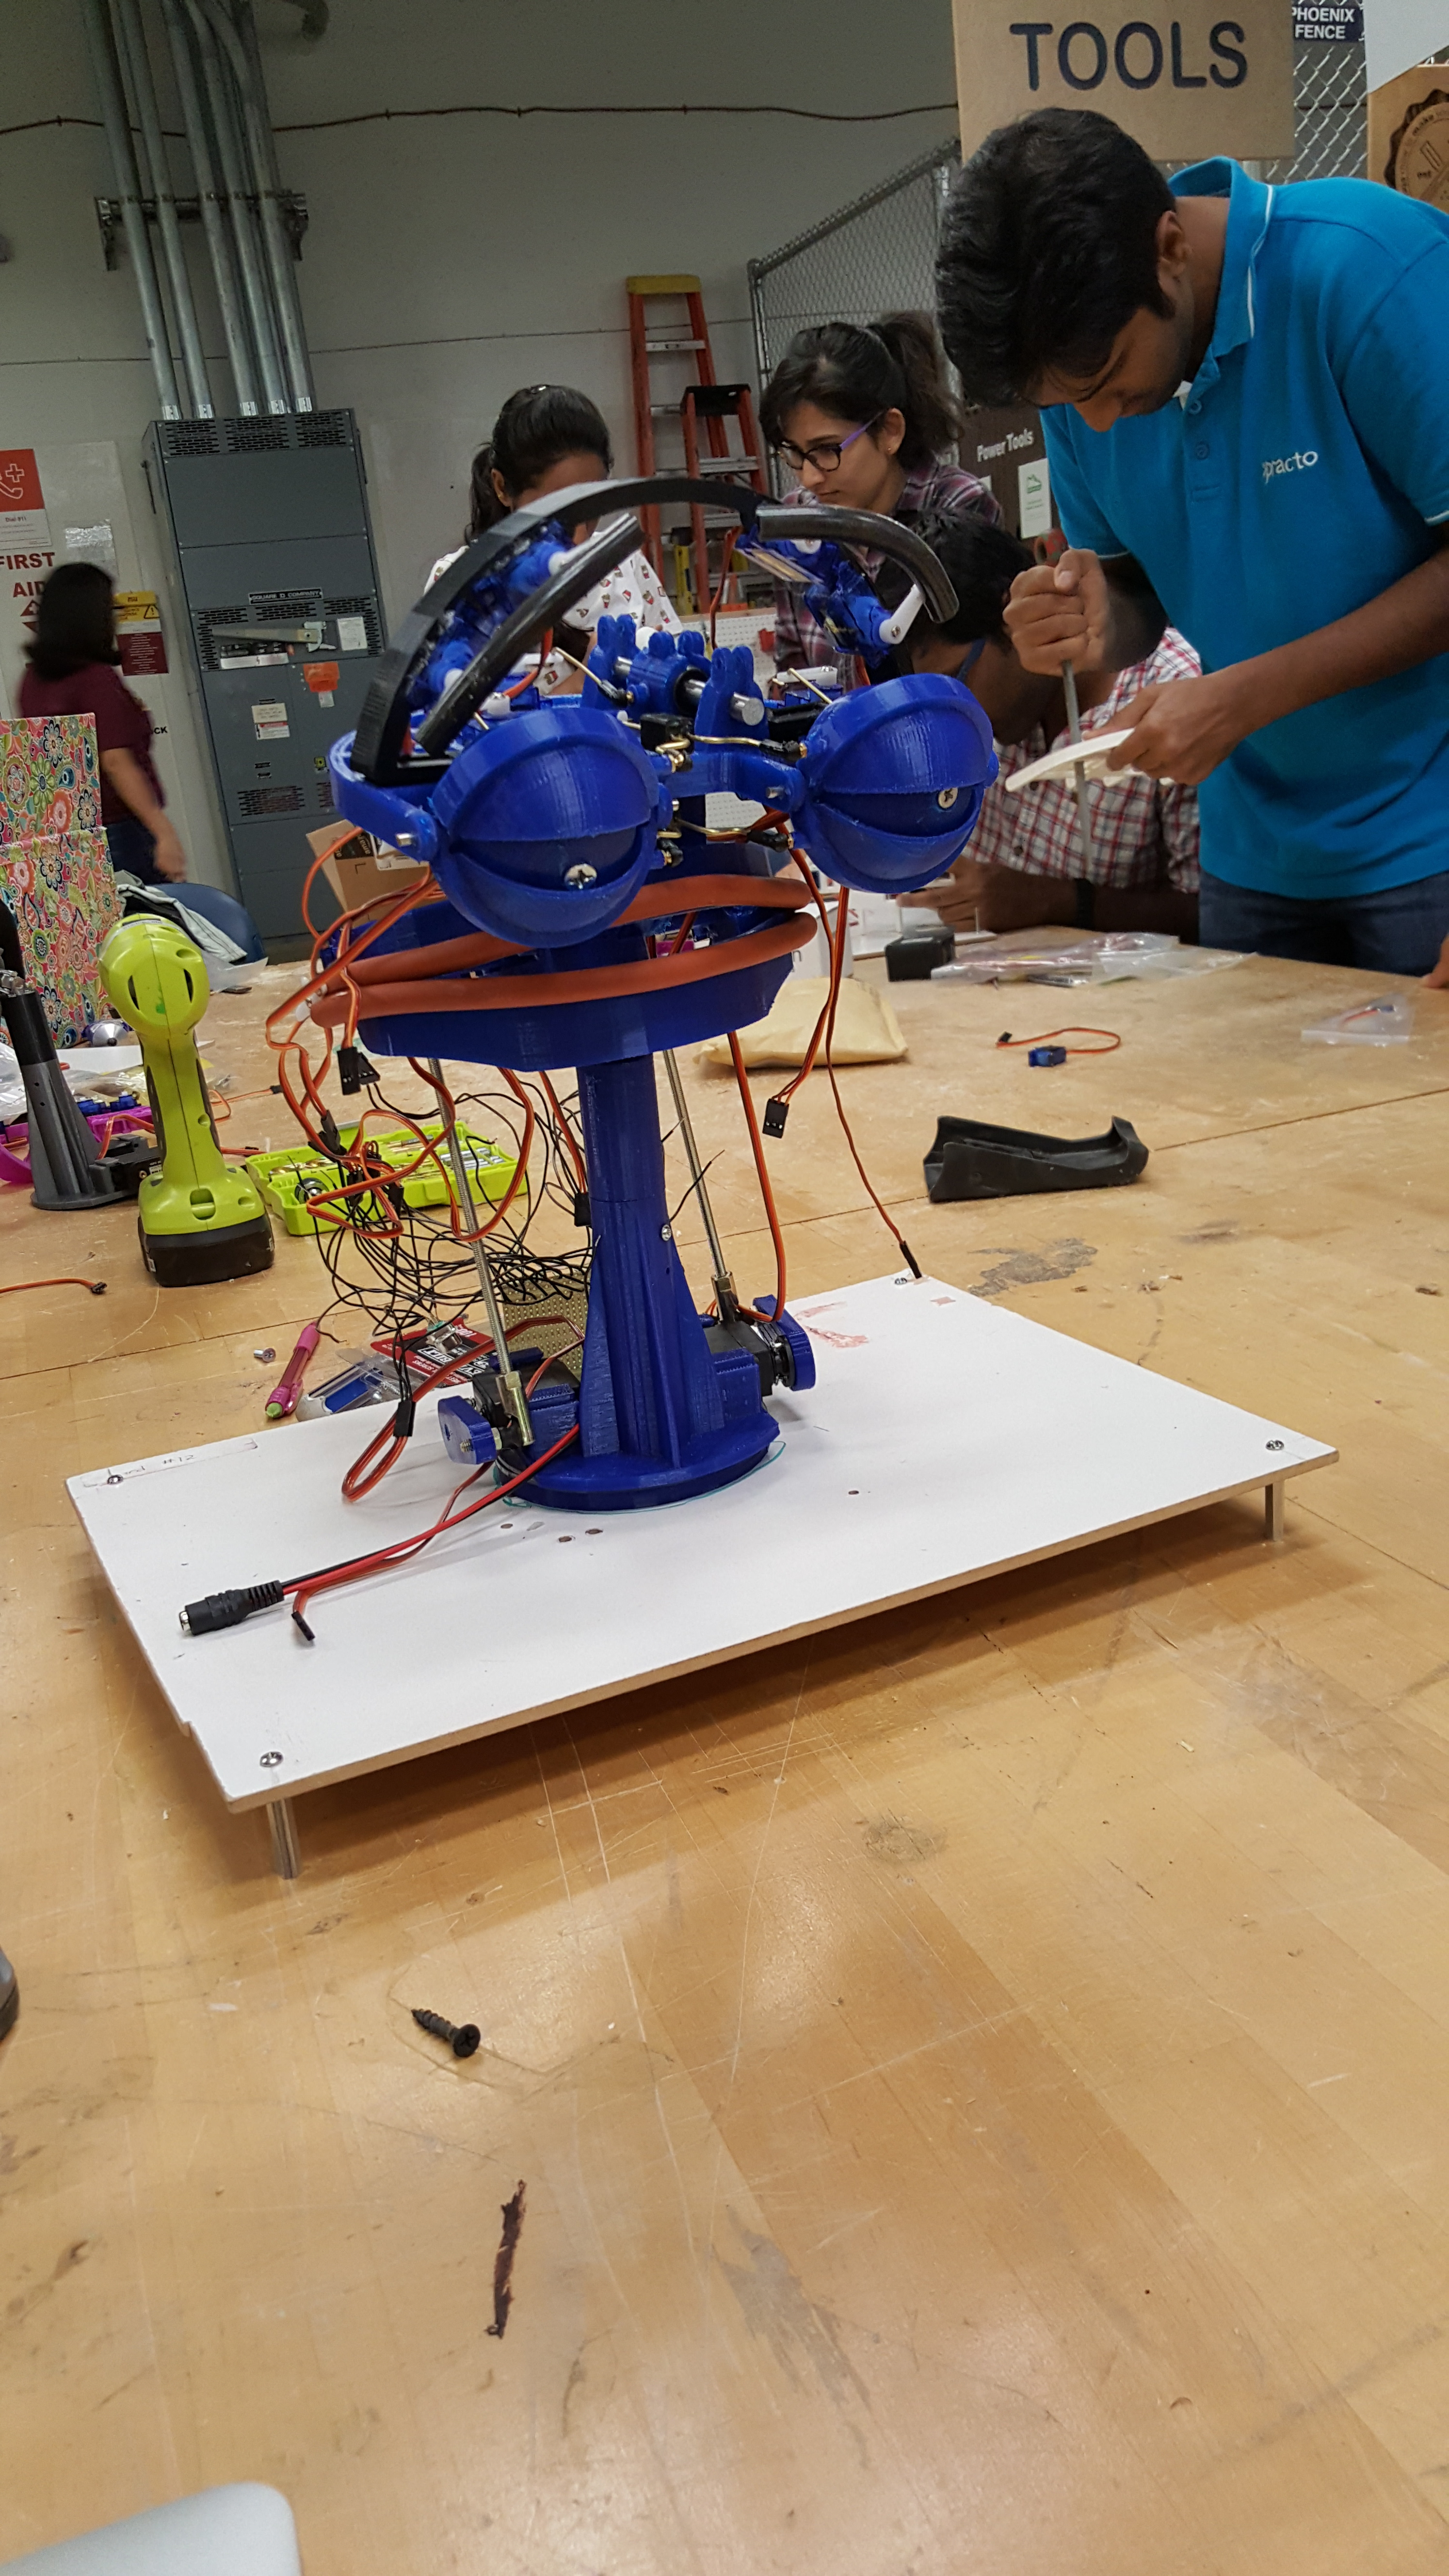
\includegraphics[width=.42\linewidth]{completed}
  \caption{Completed front}
  \label{fig:completed_robot_a}
\end{subfigure}%
\begin{subfigure}{.5\textwidth}
  \centering
  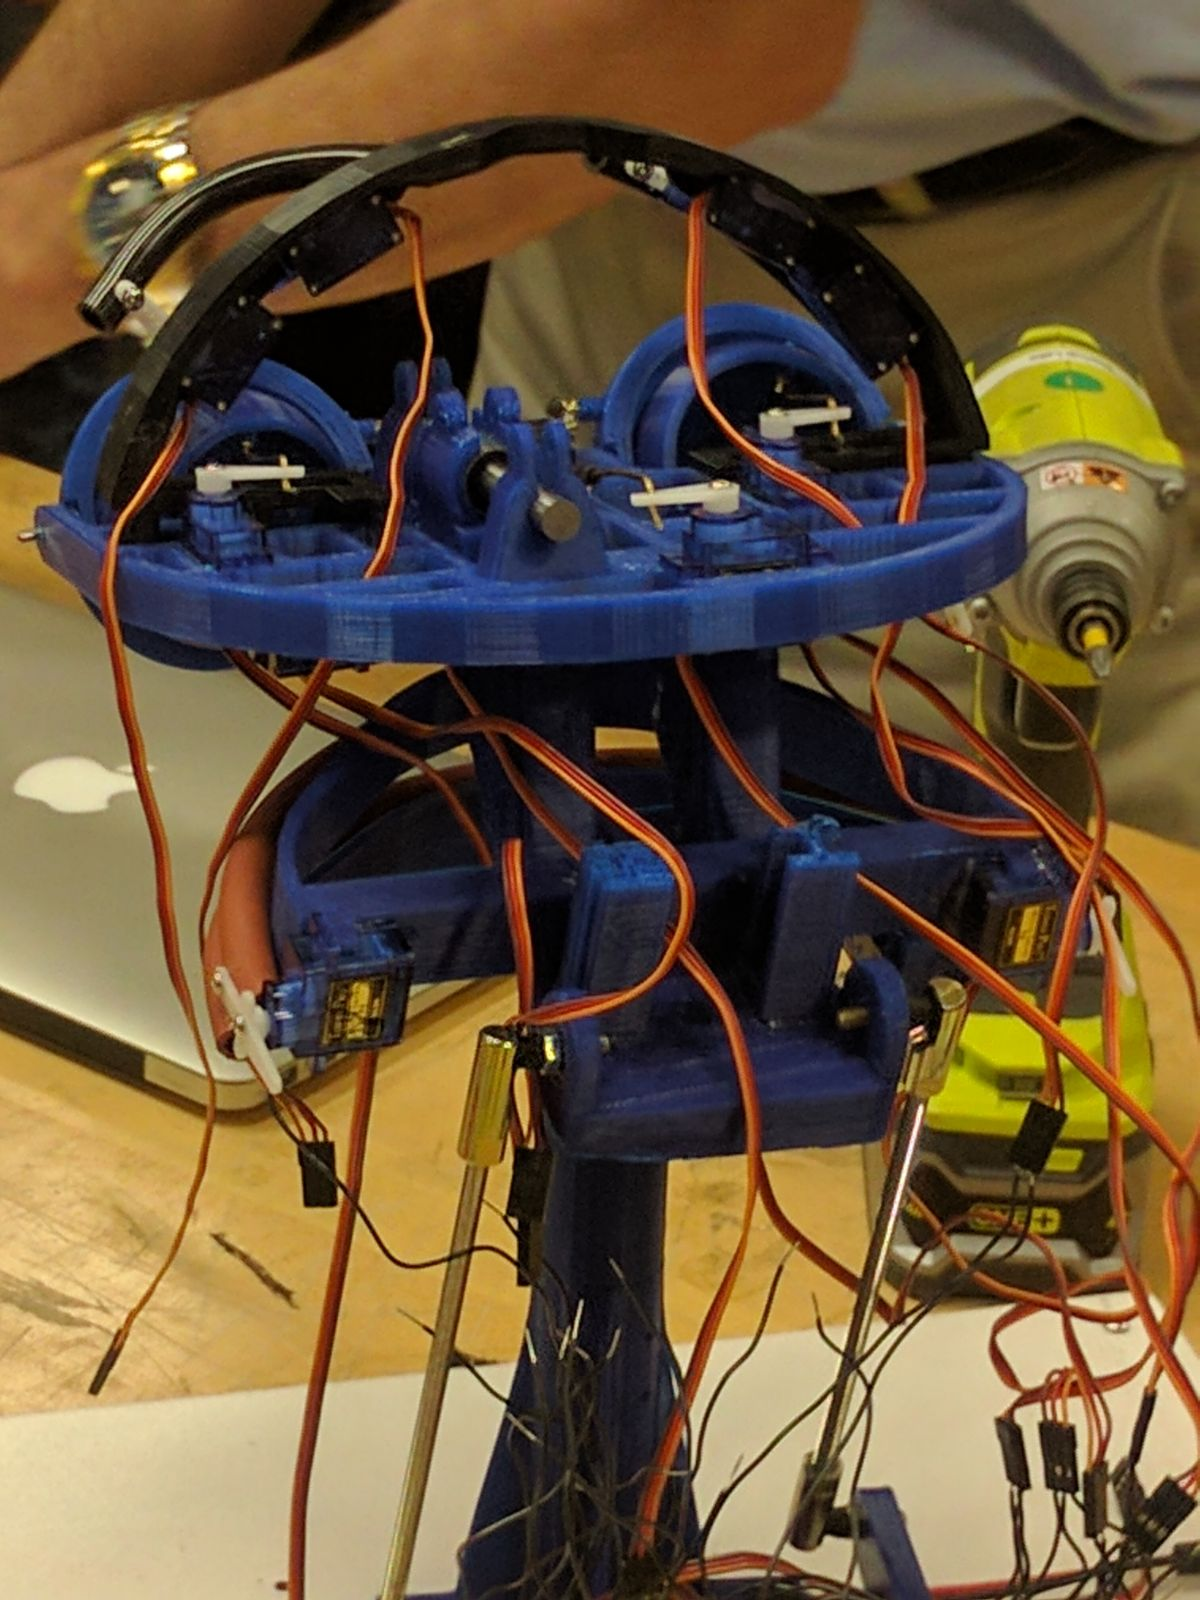
\includegraphics[width=.55\linewidth]{completed_back}
  \caption{Completed back}
  \label{fig:completed_robot_b}
\end{subfigure}
\caption{Completed robot example.}
\label{fig:completed_robot}
\end{figure}
%-----------------------------------------

{\let\clearpage\relax \labday{29 August 2016}}

\experiment{Team to Team Collaboration} We made sure that everyone had ordered the required parts for the robot. Some parts were arriving late but it was manageable as we did not require all of them at once. We also learnt about team to team collaboration. Some team members stayed in the class to figure out the blueprint and robot design while the others went to the lab to understand the 3D printing. Figure \ref{fig:blue_print} shows the most abstract idea of all the motors in the robot.

\begin{figure}[H] % Example of including images
\begin{center}
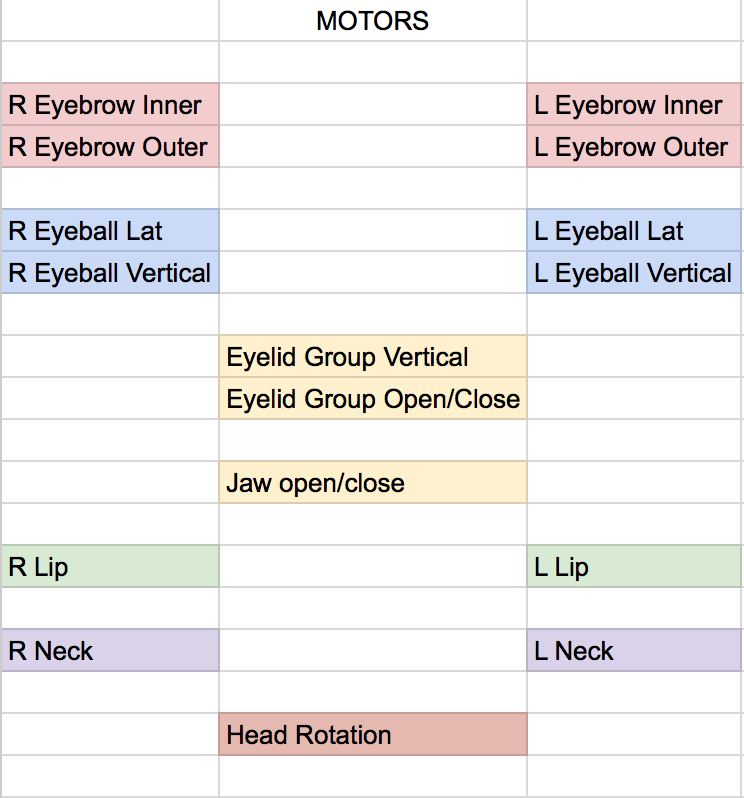
\includegraphics[width=0.5\linewidth]{blue_print}
\end{center}
\caption{Basic blueprint of the motors.}
\label{fig:blue_print}
\end{figure}

%----------------------------------------------------------------------------------------

{\let\clearpage\relax \labday{31 August 2016}}

\experiment{Introduction to 3D printing}
We were introduced to the 3D printing lab and we saw how a 3D printer works. We were given a training session which informed us what kind of plastic to use, what precision to use and what are the things we need to take care of. The plastic should be of good quality such that it comes of easily from the board and does not leave a residue. We were told how to set the temperature of the 3D printer such that the plastic solidifies before it's shape is distorted.
Figure \ref{fig:3dprinter} shows a 3D printer in action.
\begin{figure}[H] % Example of including images
\begin{subfigure}{.5\textwidth}
  \centering
  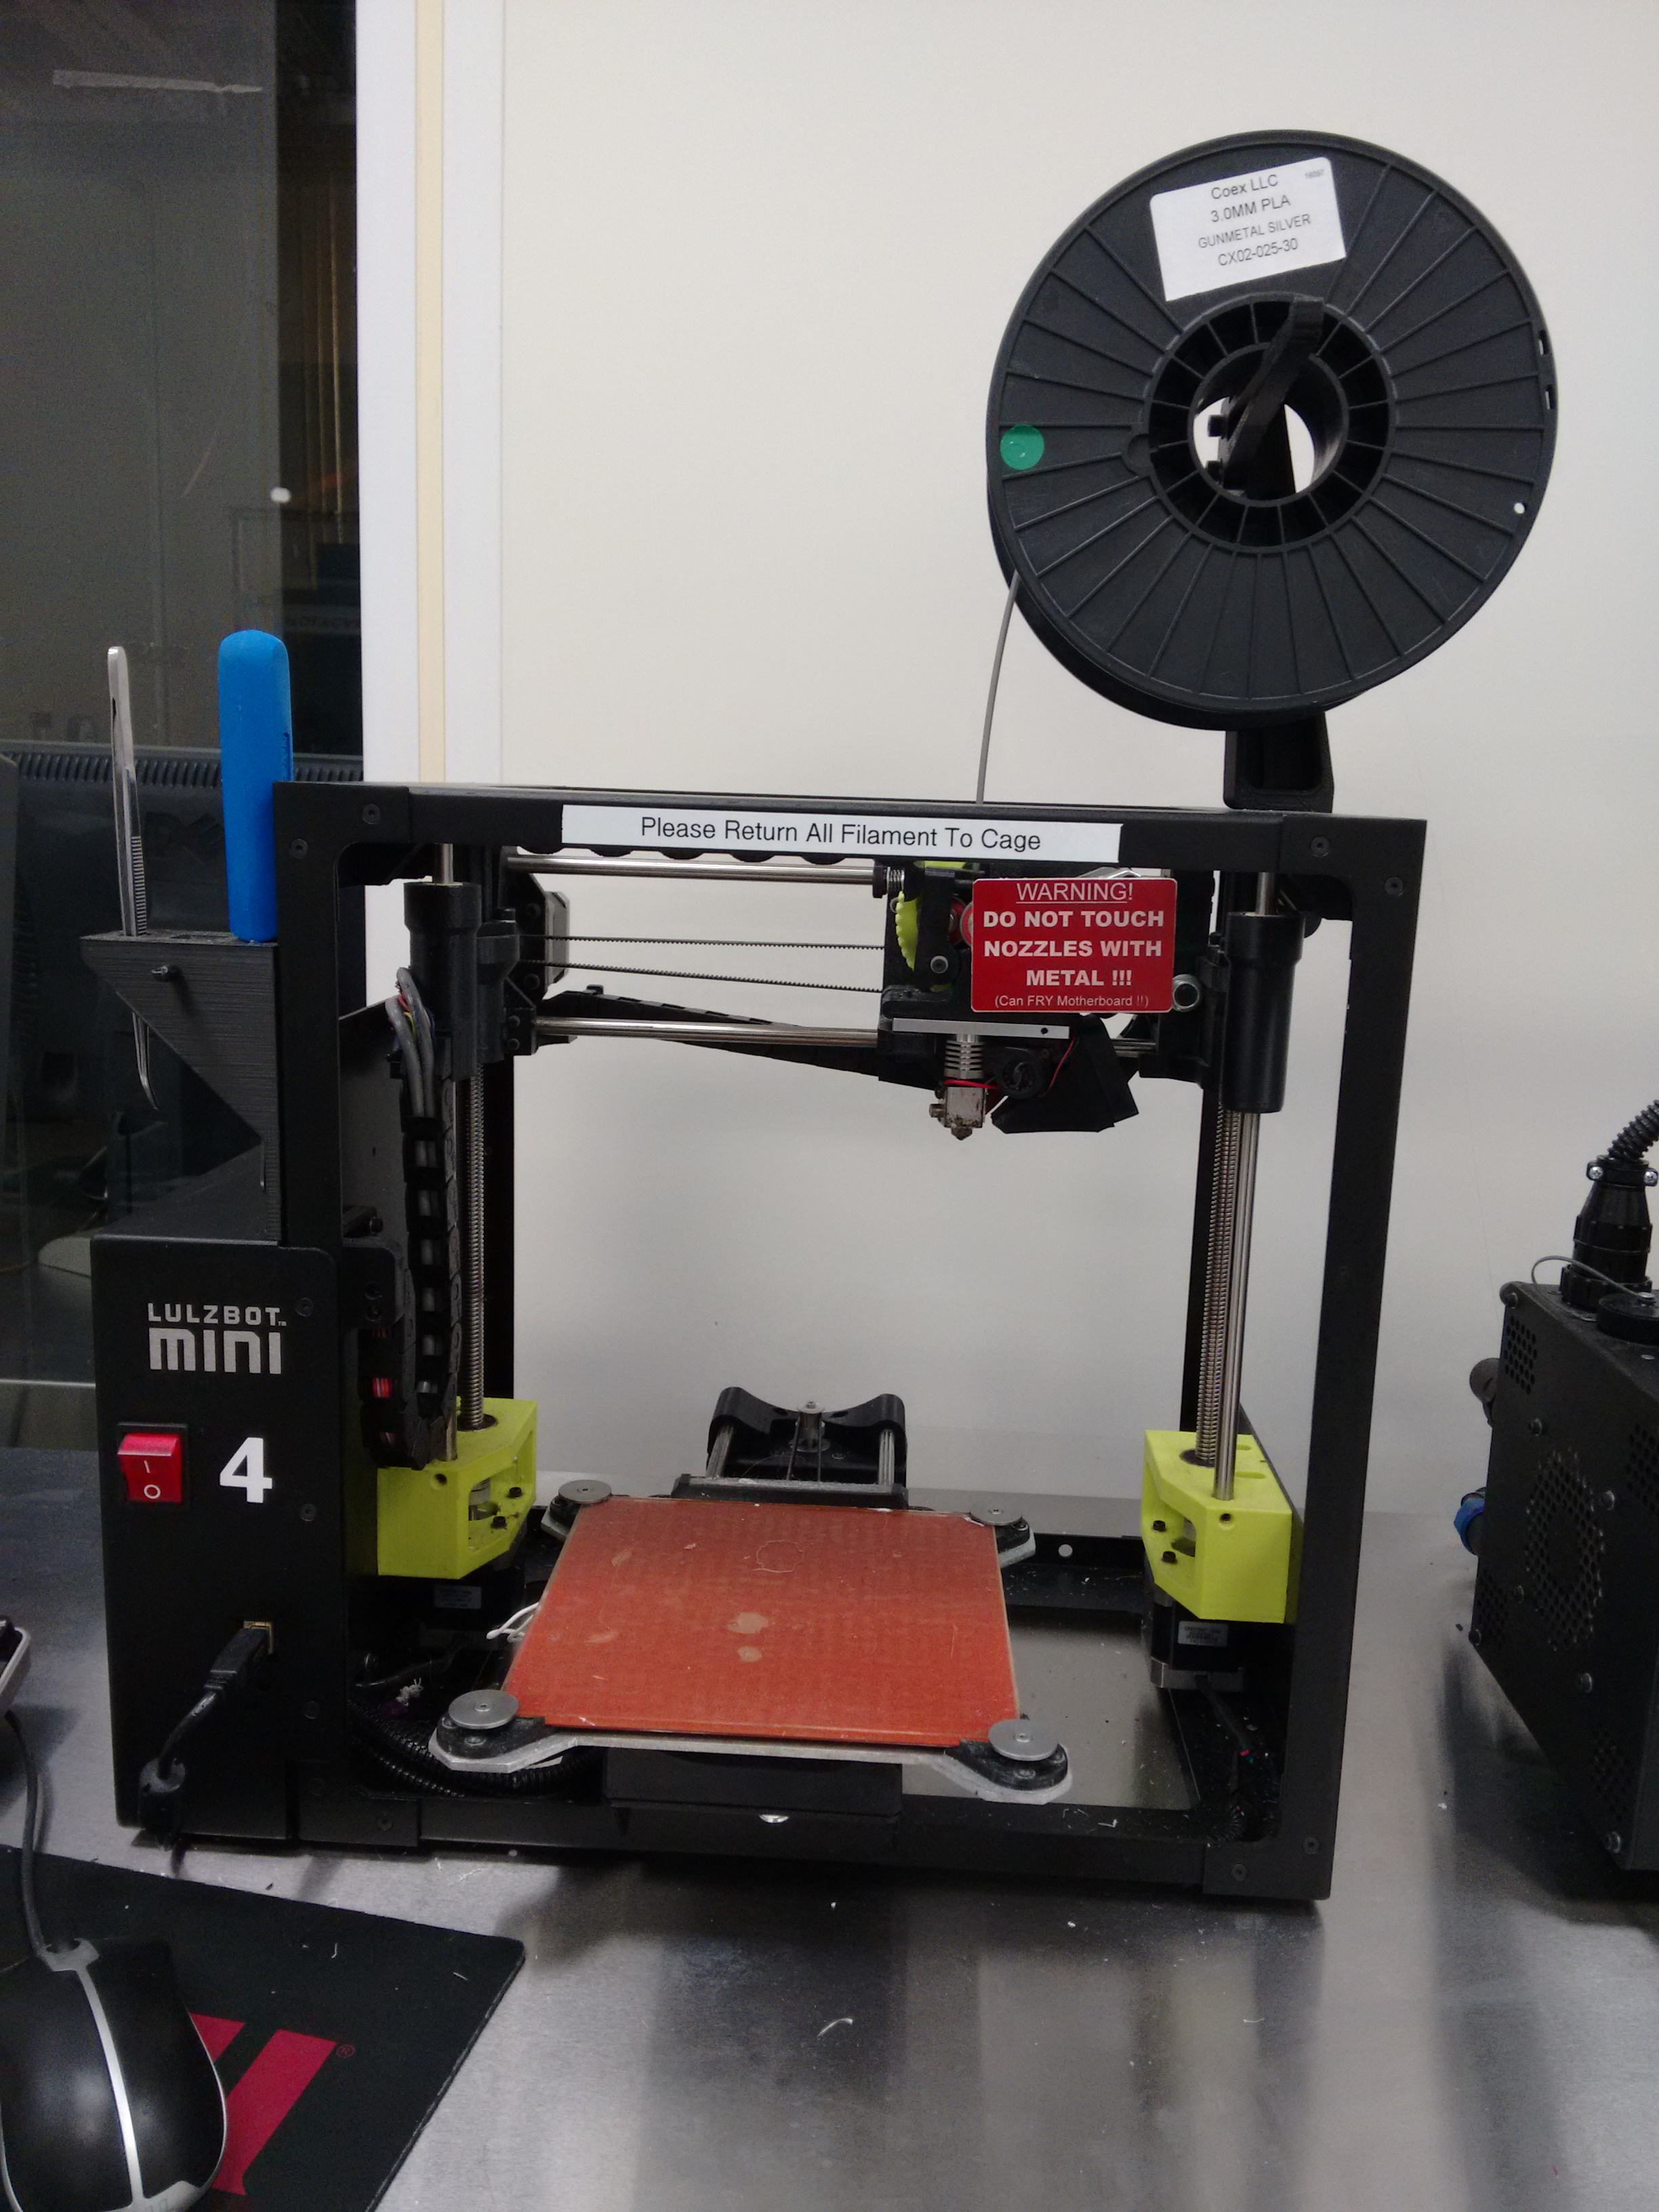
\includegraphics[width=.5\linewidth]{3d_printer}
  \caption{A 3D printer}
  \label{fig:3d_printer}
\end{subfigure}%
\begin{subfigure}{.5\textwidth}
  \centering
  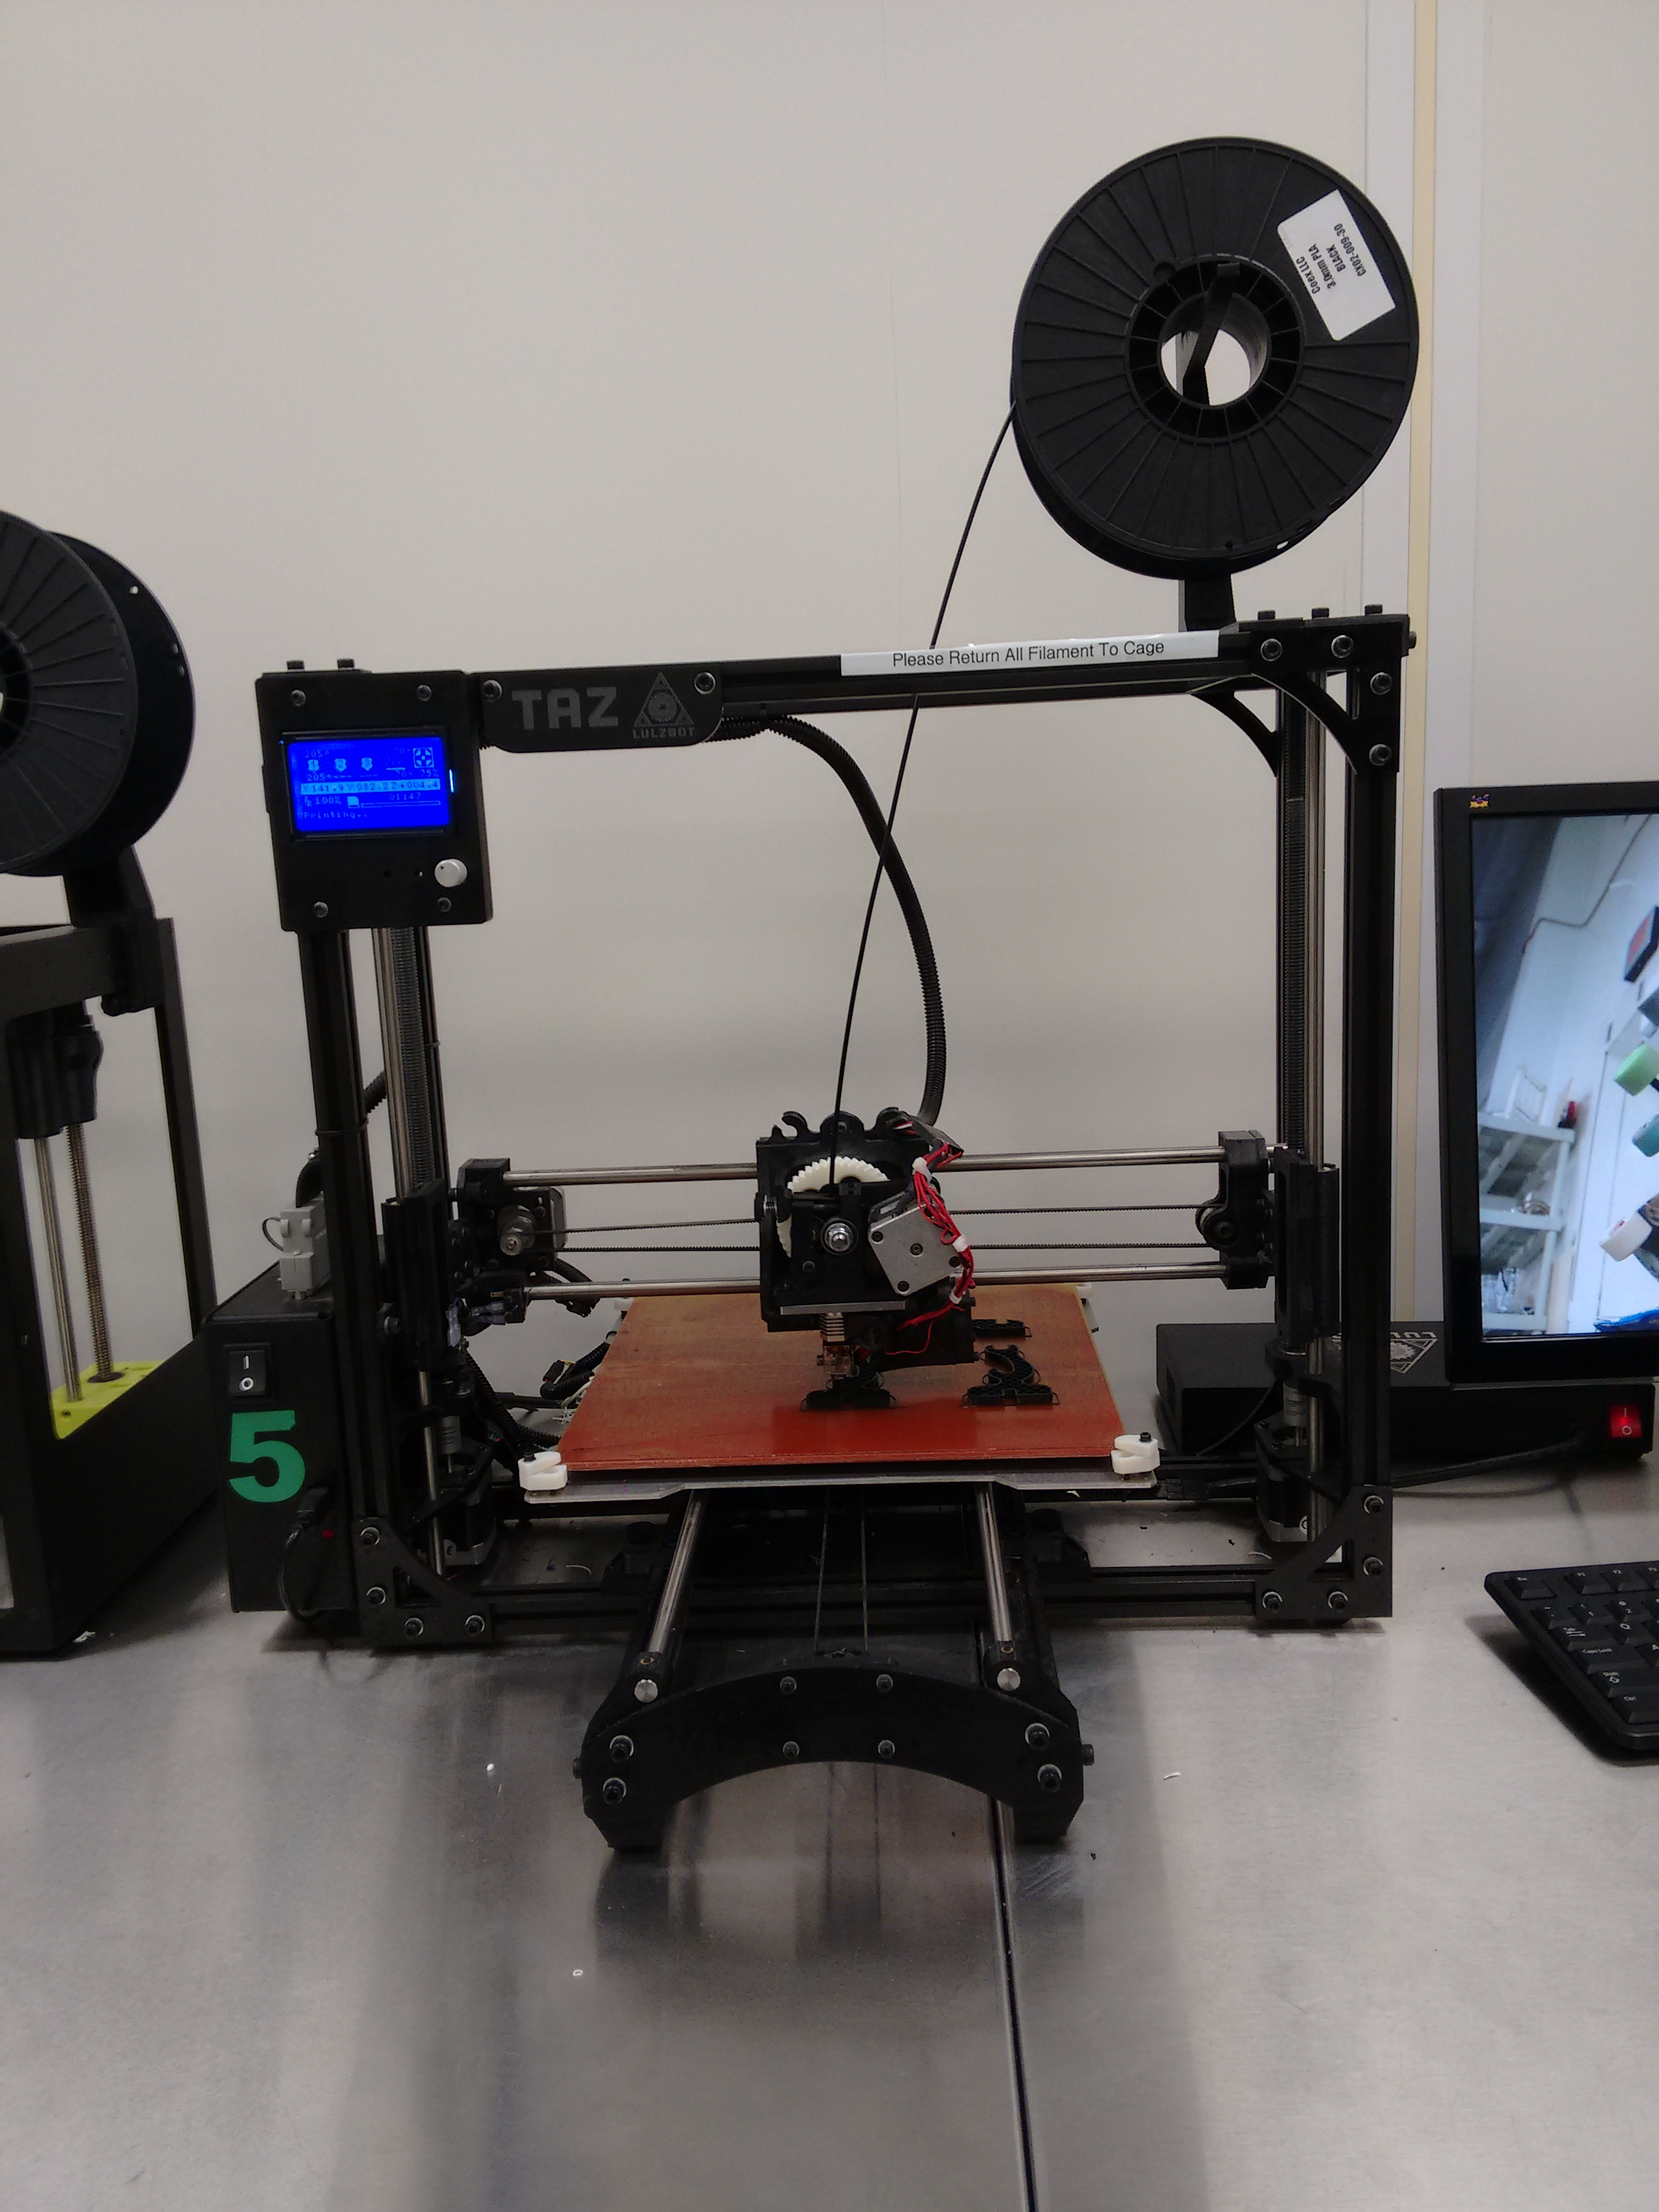
\includegraphics[width=.5\linewidth]{3d_printer_in_progress}
  \caption{3D printer in action}
  \label{fig:3d_printer_in_progress}
\end{subfigure}
\caption{A 3D printer.}
\label{fig:3dprinter}
\end{figure}

\experiment{Started printing the parts}
We booked a slot on 2nd October 2016 and started printing out the 3D parts.

%----------------------------------------------------------------------------------------

{\let\clearpage\relax \labday{7 September 2016}}

\experiment{Removing the support material}
We got some of our parts printed, while for the others we required a 3D printer with a larger board. We booked a slot for it on the 9$^{th}$ Septemper.\\
A 3D printer can print easily in 2 dimesions, but sometimes we need to print a loop or a hole. This means that the plastic does not have anything to support it. The 3D printer prints an extra supporting material which needs to be removed once the printing is complete. Some of our parts had this supporting material and we worked on scraping of this material from our parts. We used pliers and filers to remove it and smoothen our parts.

%----------------------------------------------------------------------------------------

{\let\clearpage\relax \labday{12,14 September 2016}}

\experiment{Drilling of neck joint}
The robot has a neck which should be freely movable in all the directions, just like a human neck. To make this happen we had ordered a universal joint. But this joint was not fitting inside the neck as the 3D printer was not a high precision printer. To make that happen, we used a drill bit of $1.34cm$. This part was inserted in the base, which was again drilled. The final setup looked somewhat like \ref{fig:neck_joint}.

\begin{figure}[H] % Example of including images
\begin{center}
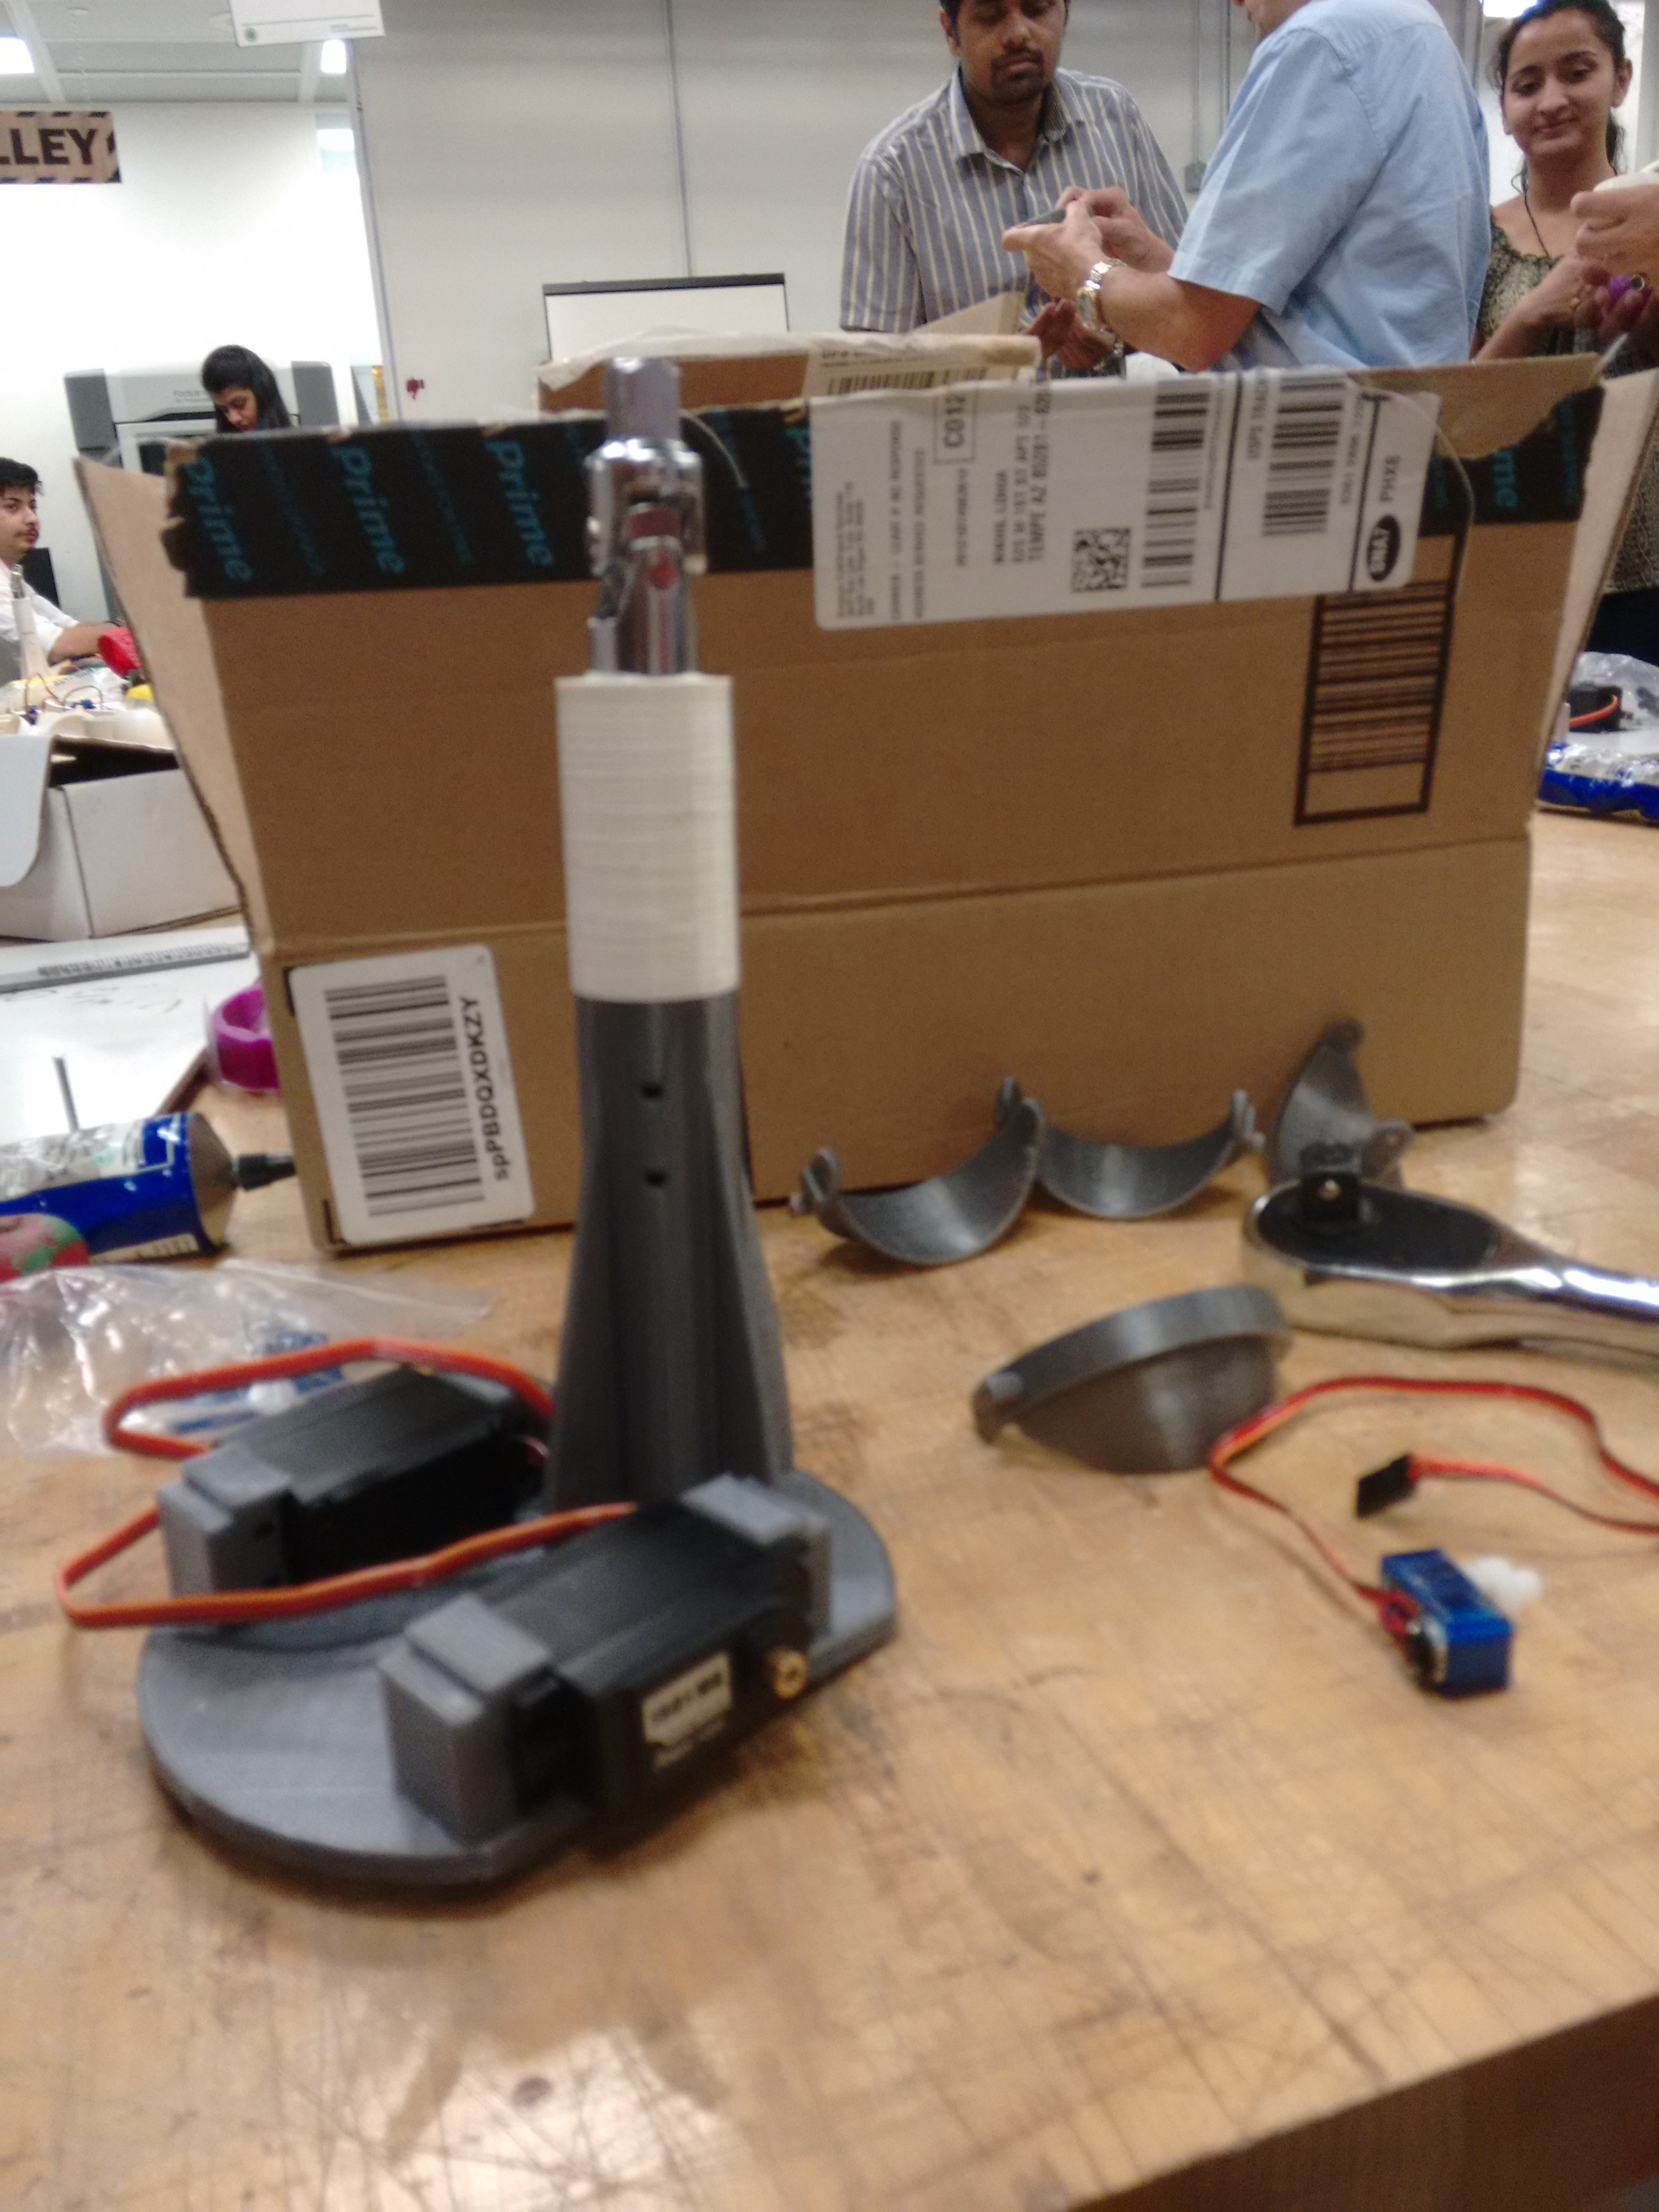
\includegraphics[width=0.4\linewidth]{neck_joint}
\end{center}
\caption{Setting up the robot neck with universal joint.}
\label{fig:neck_joint}
\end{figure}

\experiment{Filing and cleaning and drilling}
We got all our parts printed out. This meant we had to clean them of the supporting material, file them to smoothen it and drill some holes so other parts could fit properly. This day of the lab was majorly based upon collaborating with each other and learning from the professor.

\begin{figure}[H] % Example of including images
\begin{center}
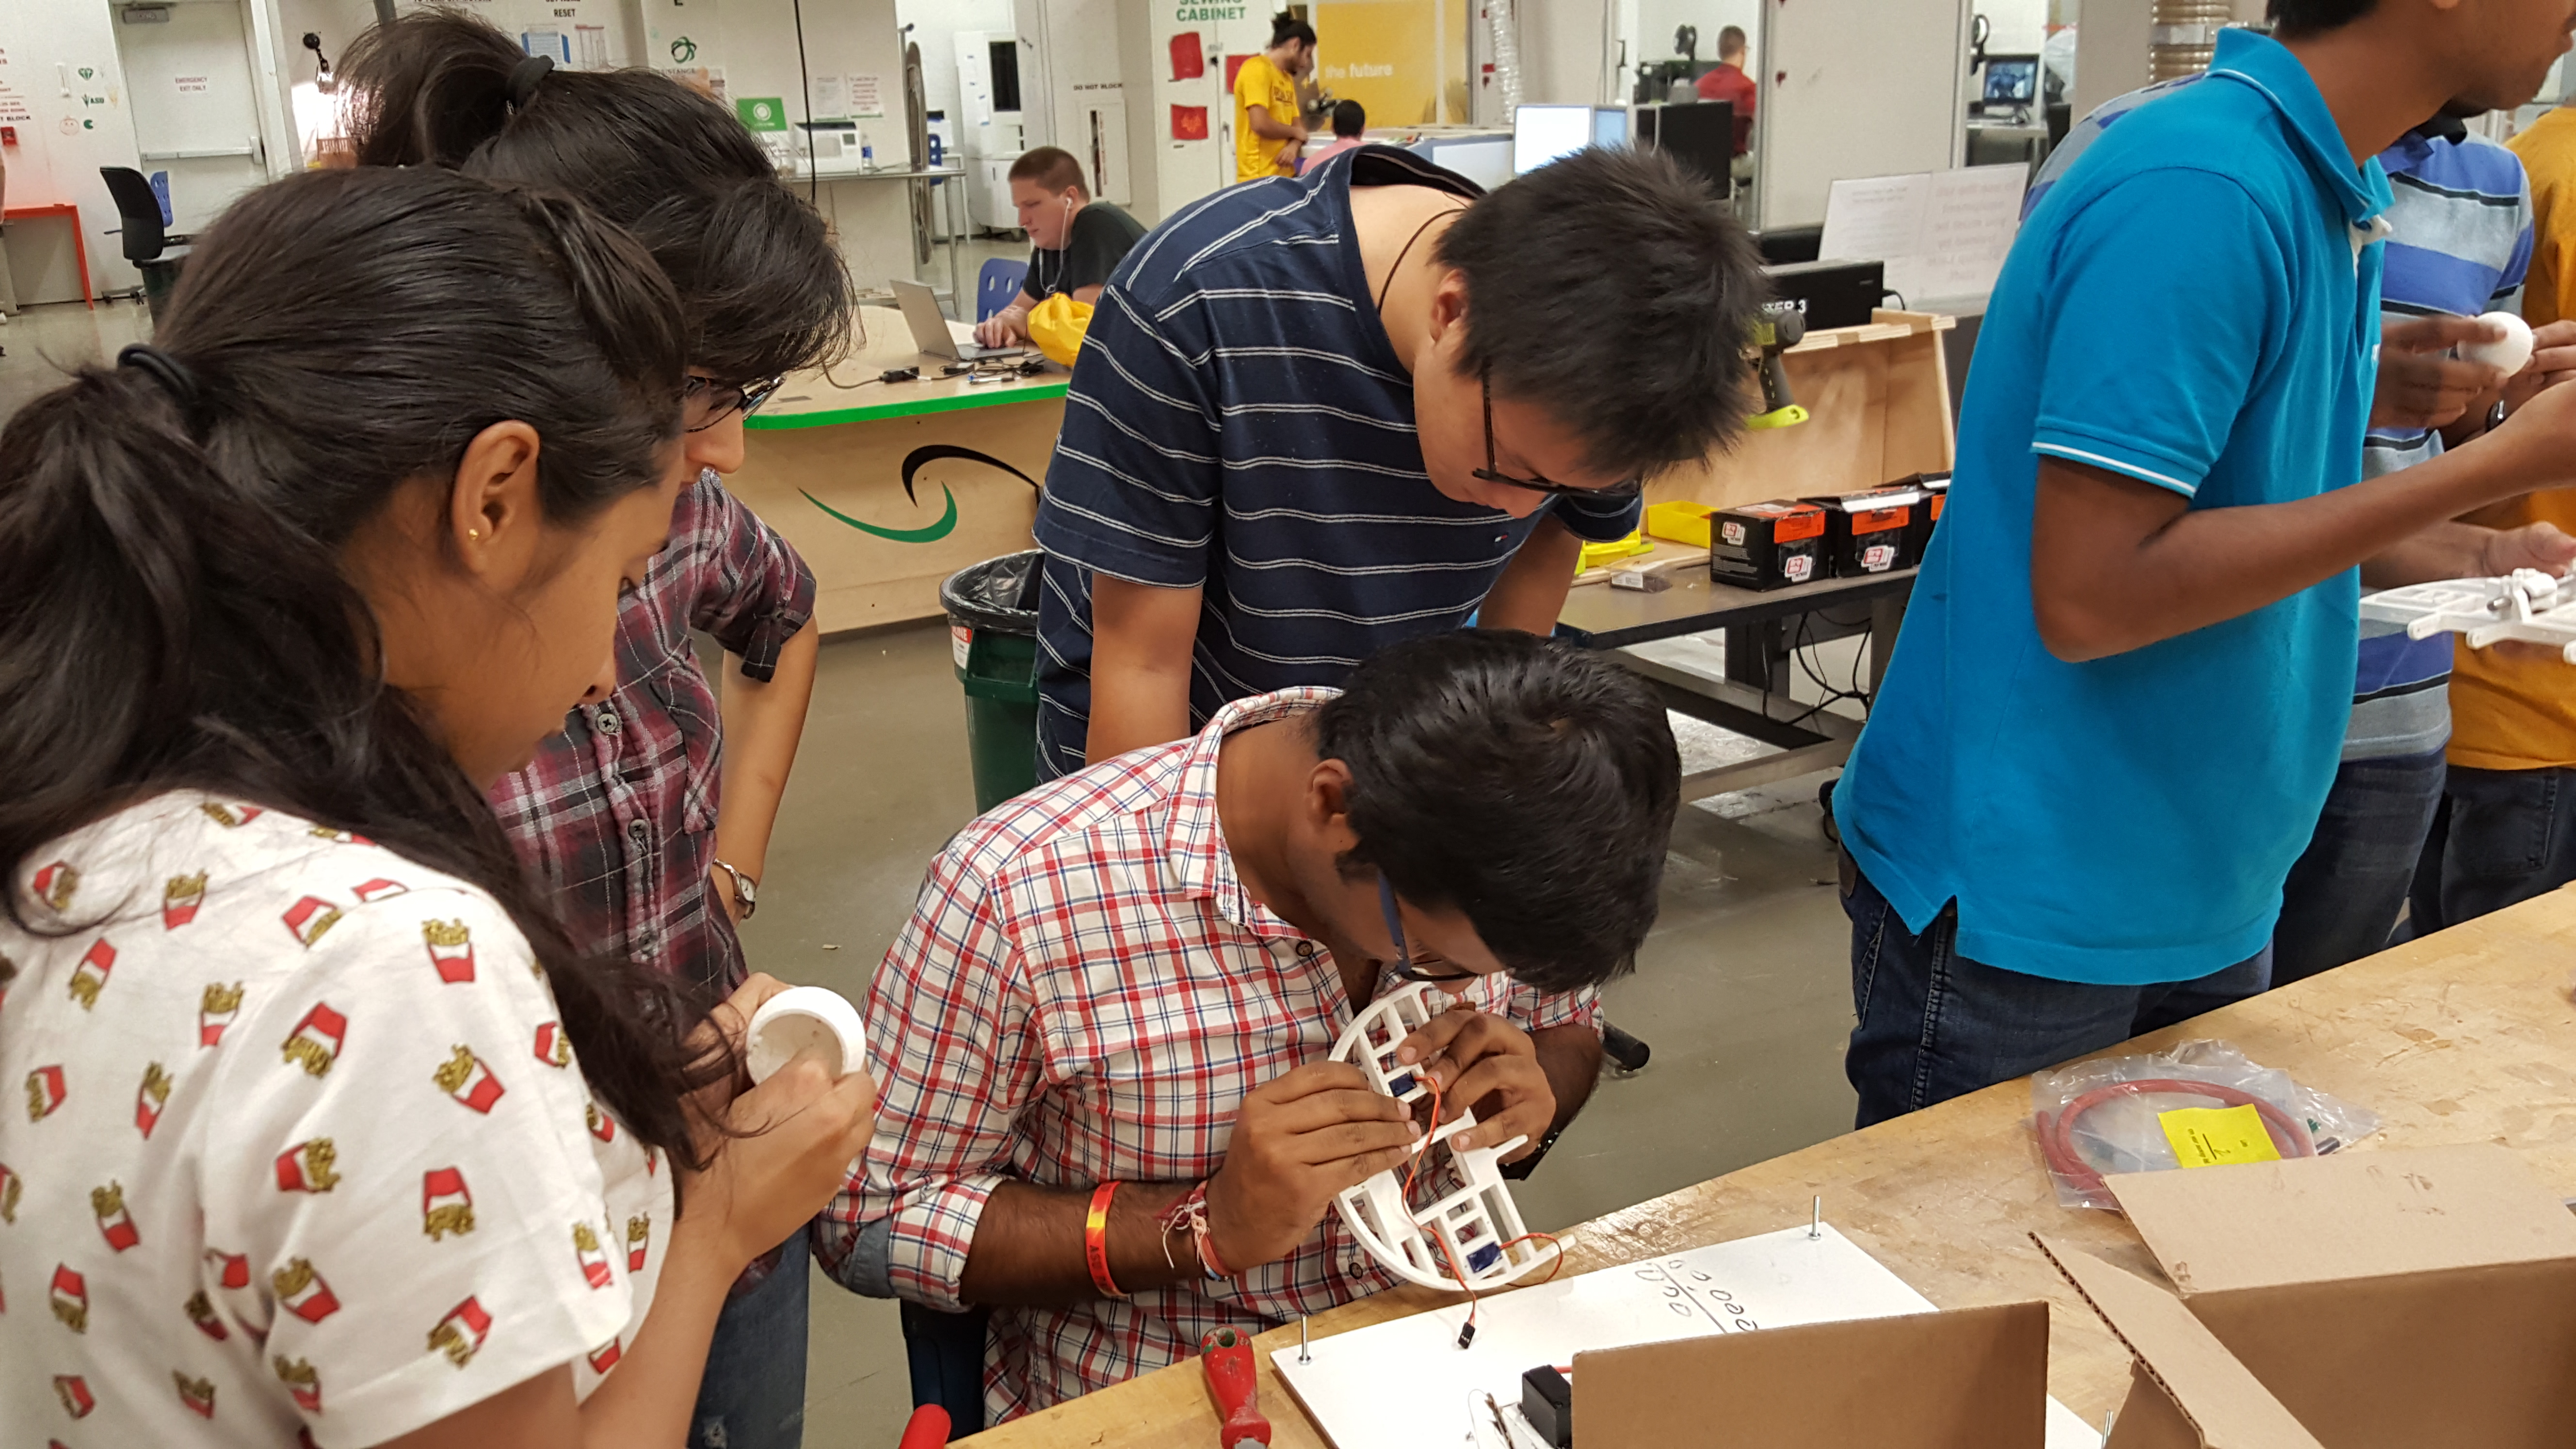
\includegraphics[width=0.4\linewidth]{work_in_progress}
\end{center}
\caption{Working together as a team.}
\label{fig:work_in_progress}
\end{figure}

%----------------------------------------------------------------------------------------

{\let\clearpage\relax \labday{19 September 2016}}

\experiment{Fitting of servo motors in base}
We started fitting the servo motors in the robot base. This would enable our robot to tilt its face in the left and right direction. This will be achieved by the use of 32 $*$ 6$''$ threaded rods which would be attached on both the sides of the servo motors. Figure \ref{fig:robo_neck_mouth} shows how the rods and the motors were connected to the base.

\experiment{Fitting of servo motors in head}
The eyebrows of the robot will also be controlled by the servo motors. For this we took the head of the robot and filed it so that our motors could fit inside it. Once the cut was made appropriate to the motors, we affixed the motors and ensured that their directions were opposite. This would enable a greater movement of the eyebrows. We will need to initialize the servo motors to their starting positions once we start programming our robot. Figure \ref{fig:robo_head_servos} shows how the servo motors are connected in the head.

\begin{figure}[H] % Example of including images
\begin{subfigure}{.5\textwidth}
  \centering
  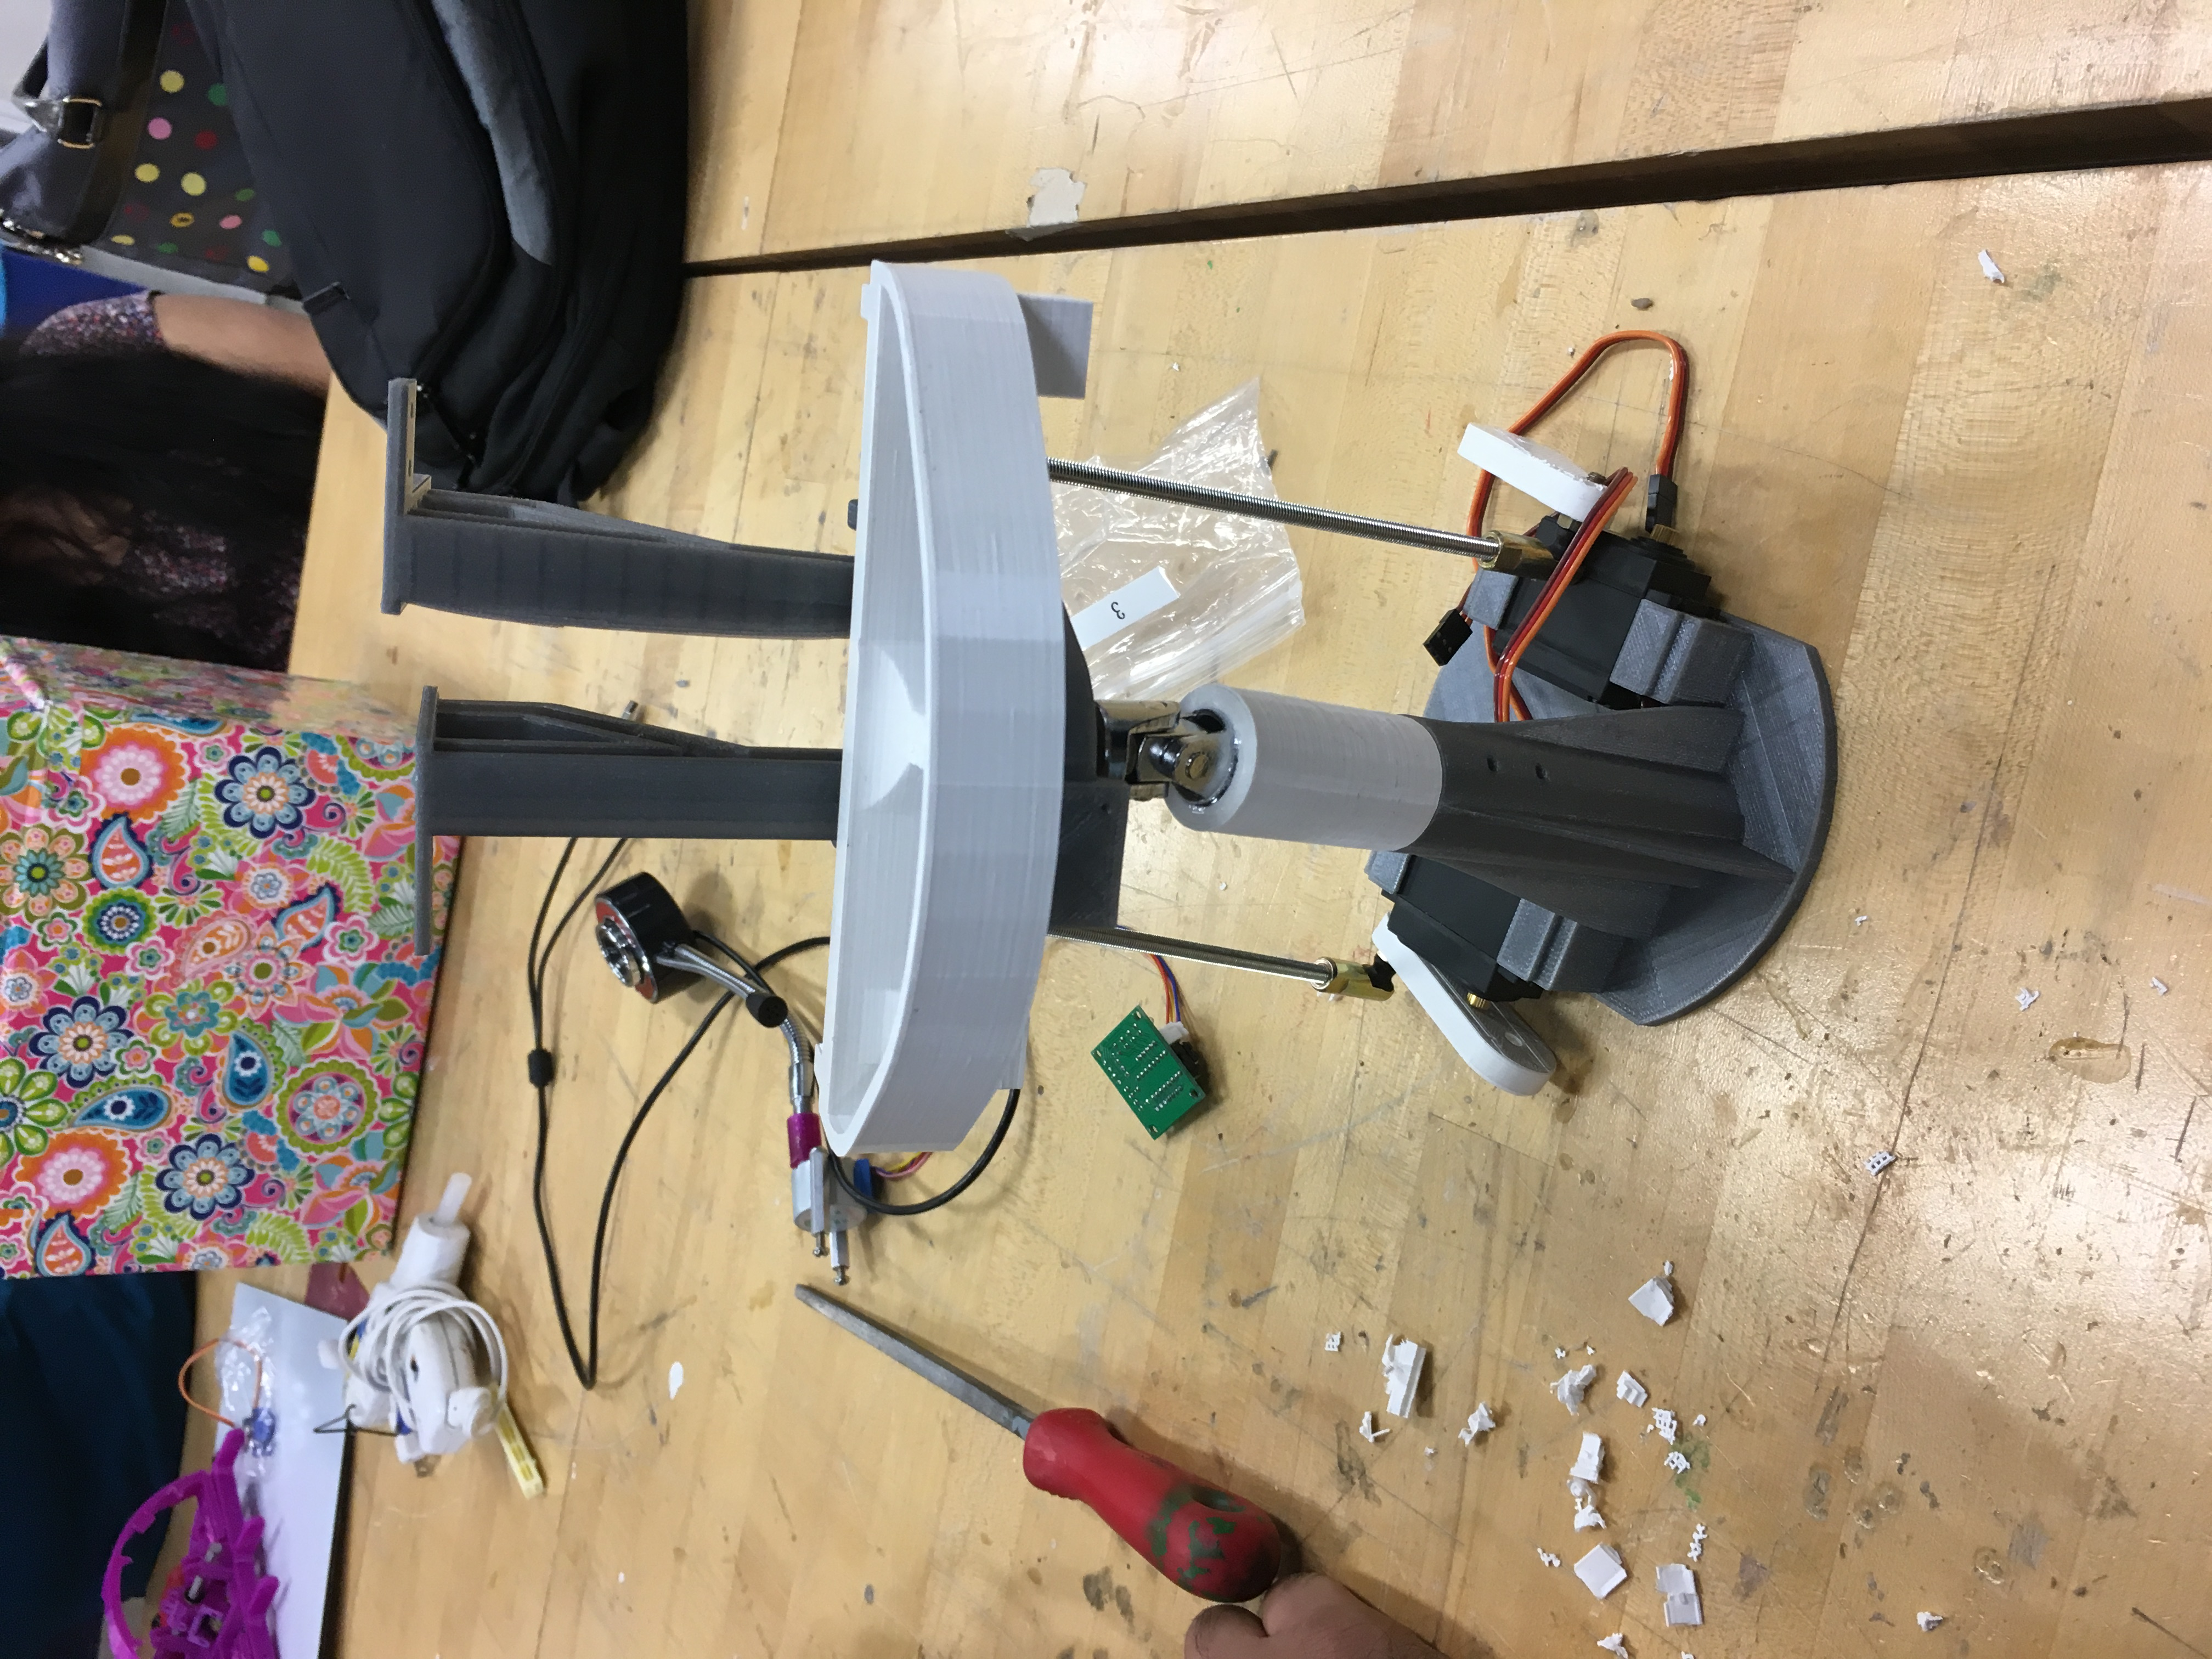
\includegraphics[width=.65\linewidth, angle=-90]{robo_neck_mouth}
  \caption{Robot with servo motors in base}
  \label{fig:robo_neck_mouth}
\end{subfigure}%
\begin{subfigure}{.5\textwidth}
  \centering
  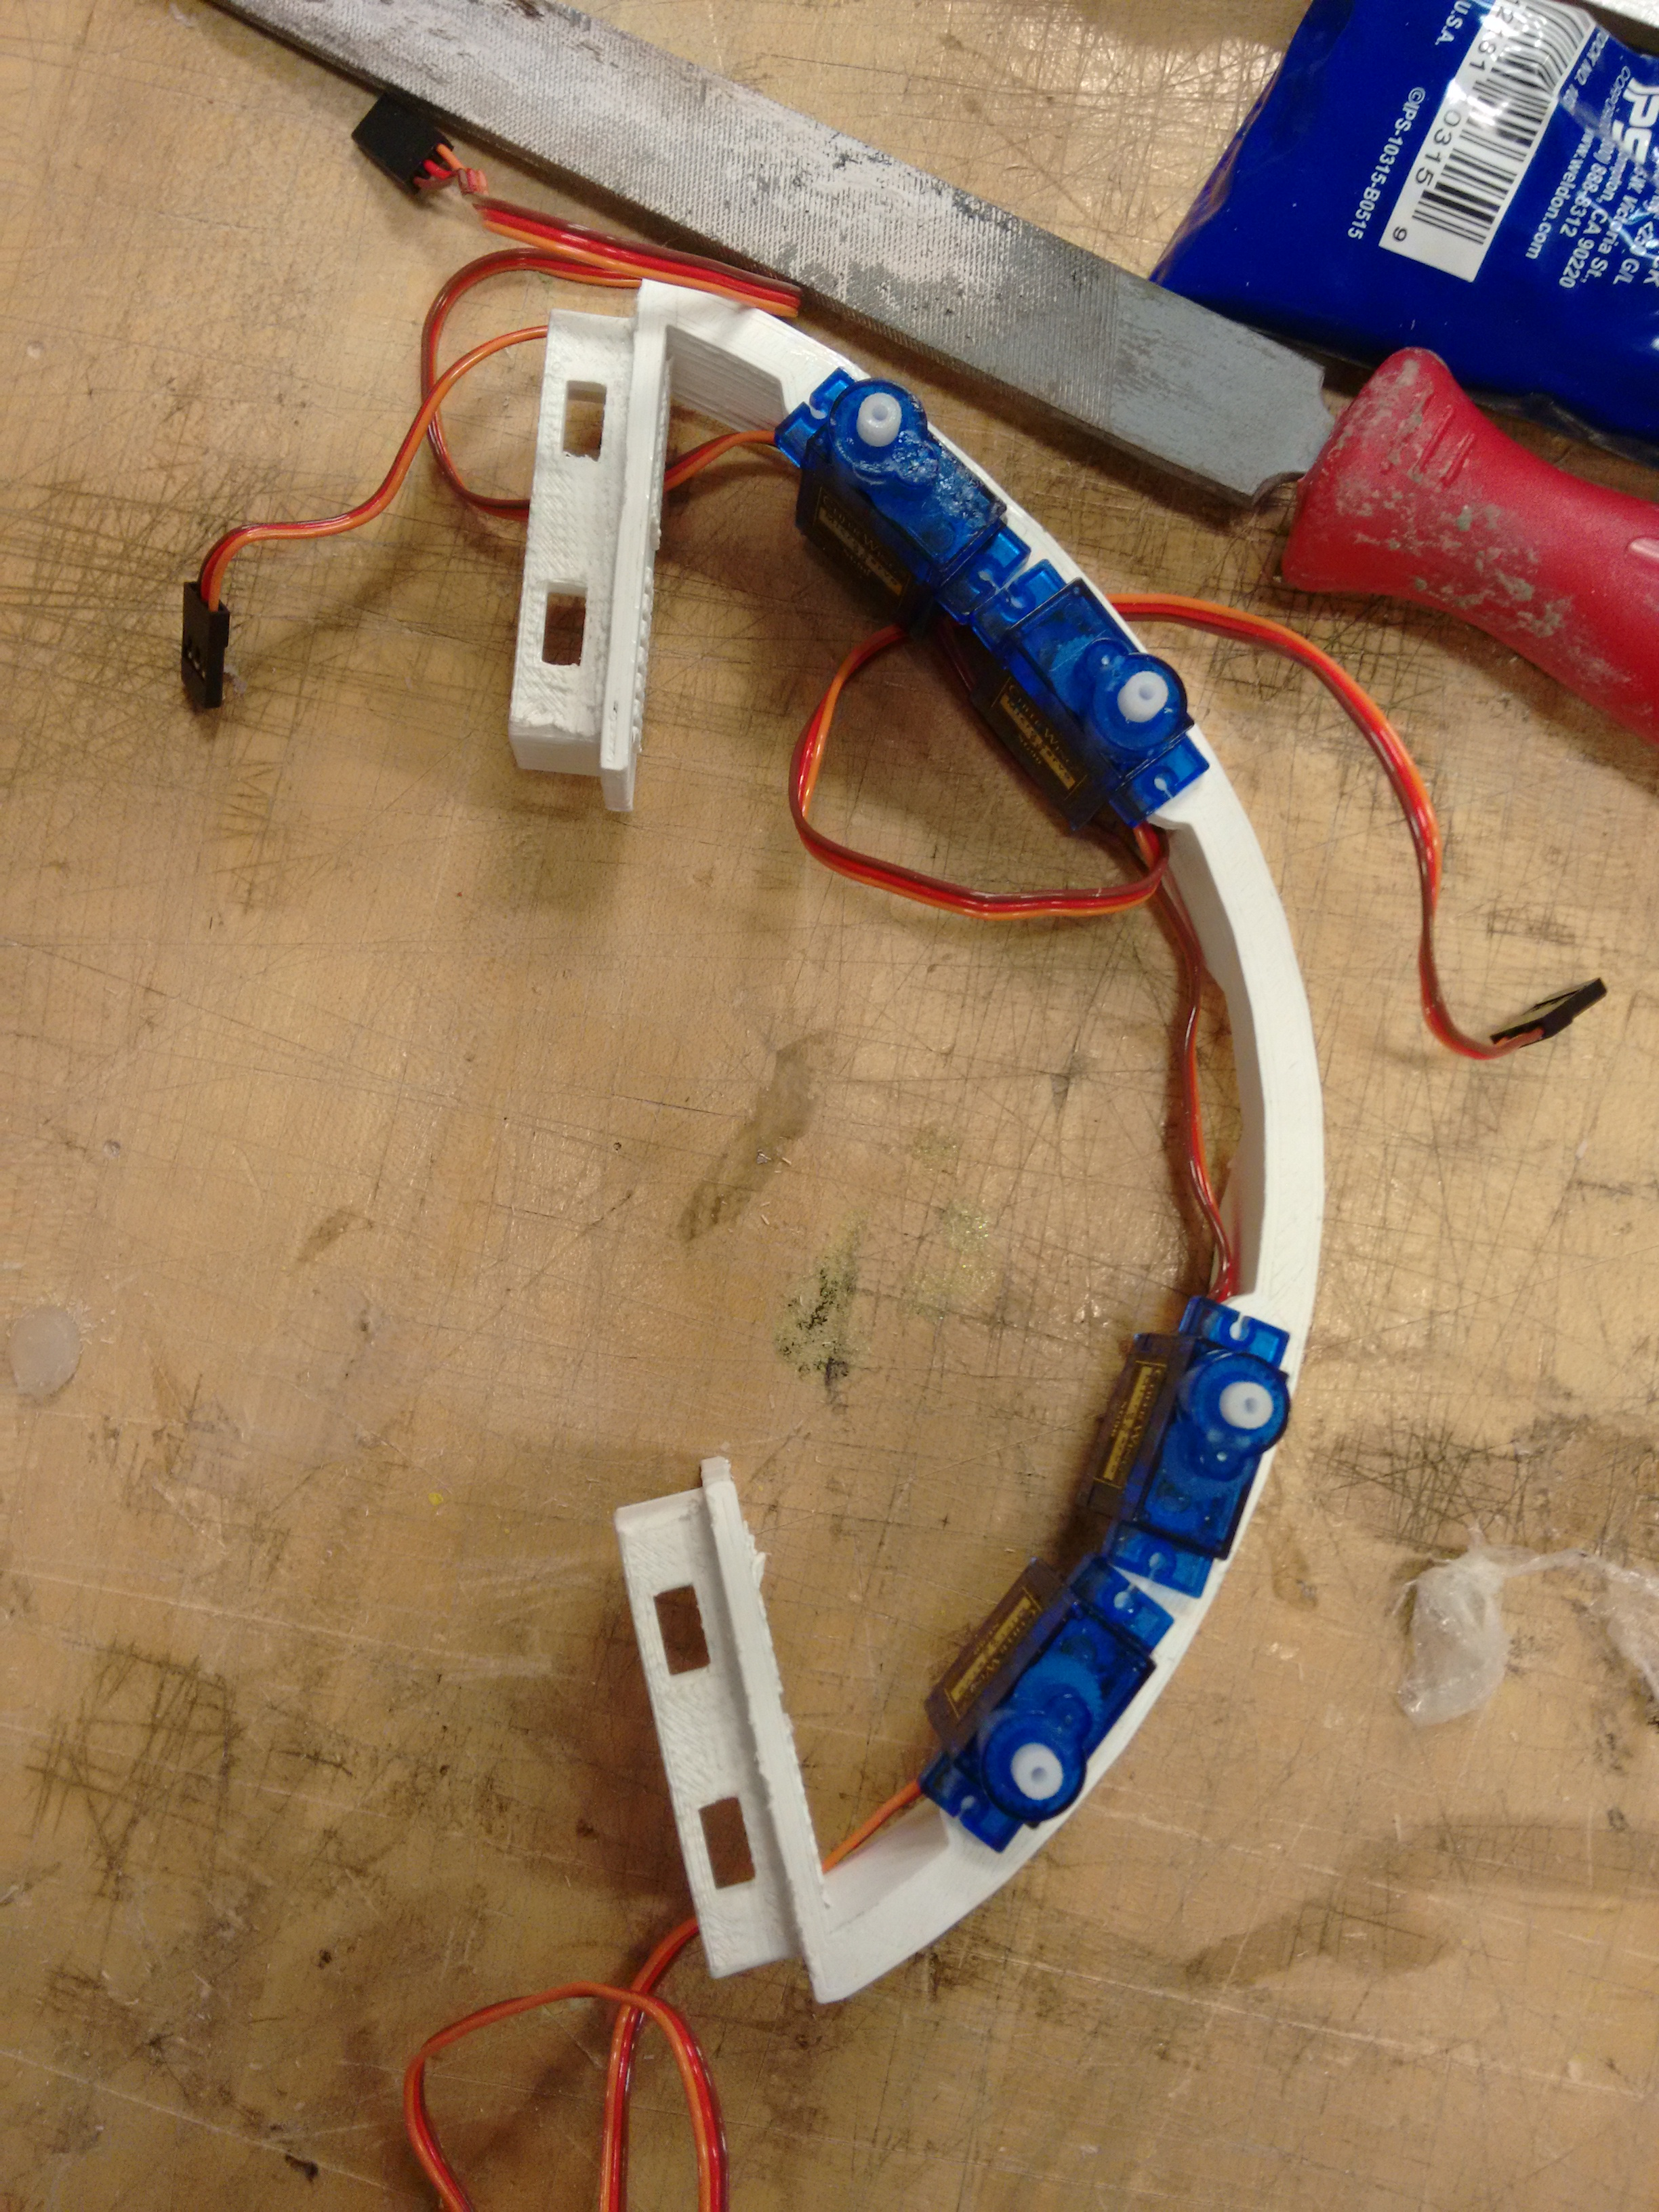
\includegraphics[width=.5\linewidth]{robo_head_servos}
  \caption{Servo motors to control eyebrows}
  \label{fig:robo_head_servos}
\end{subfigure}
\caption{Fitting servo motors.}
\label{fig:servo_motors}
\end{figure}

%----------------------------------------------------------------------------------------

{\let\clearpage\relax \labday{21 September 2016}}

\experiment{Cleaning the Eye Mechanism}
This was a tricky part because the motors could not be inserted directly into the eye mechanism. The wires on the side of servo motors prevented the motors from going inside directly. We could not make the holes bigger as the motor would fall. To achieve the task we filed the socket only to an extent such that the wire could go through the small file.

\experiment{Inserting the servo motors}
The servo motors were inserted in a two step process. The motor was opened and inserted from top such that the wire came down. The cap of the motor was then sealed from the other side using screws. This gave a very good fit for our servo motors. A total of $3$ motors were inserted this way.

%----------------------------------------------------------------------------------------

{\let\clearpage\relax \labday{26, 28 September 2016}}

\experiment{Drilling the eyeball}
The eye ball was cleaned and filed such that it looked like a sphere from the outside. A hole was then drilled through the plastic part which would be used to connect the eyeball U joint. This joint is held together by a screw which looks like a pupil in the eye.

\experiment{Connecting the eyelids}
The eyelids are connected using a 4mm ball connector which would be then connected to servo motors. The eyelids could now operate independently and were able to close and open.

\experiment{Connecting the U joint}
The U joint had to be made in such a way that it allowed movement in every direction. We filed the parts which enabled a smooth movement and then with the help of the professor we connected these parts together.

%----------------------------------------------------------------------------------------

{\let\clearpage\relax \labday{3 October 2016}}

\experiment{Discussion about Design}
This time we headed to the class where we discussed the use of design in various upcoming technological avenues. We discussed the use of design in the supply chain, Artificial Intelligence and Virtual reality. In this class, professor focused on the deliverables that he required from the students. We also discussed about the progress of the robot.

%----------------------------------------------------------------------------------------

{\let\clearpage\relax \labday{5 October 2016}}

\experiment{Started Gluing the parts}
We had not been gluing any of the parts as of now because of several design changes along the way. The robot is now getting into the final stage and thus we started gluing all the parts together. We started off with the motors in the head. We glued the head base with the head support and placed the base of the robot on a cardboard sheet.

\begin{figure}[H]
\begin{center}
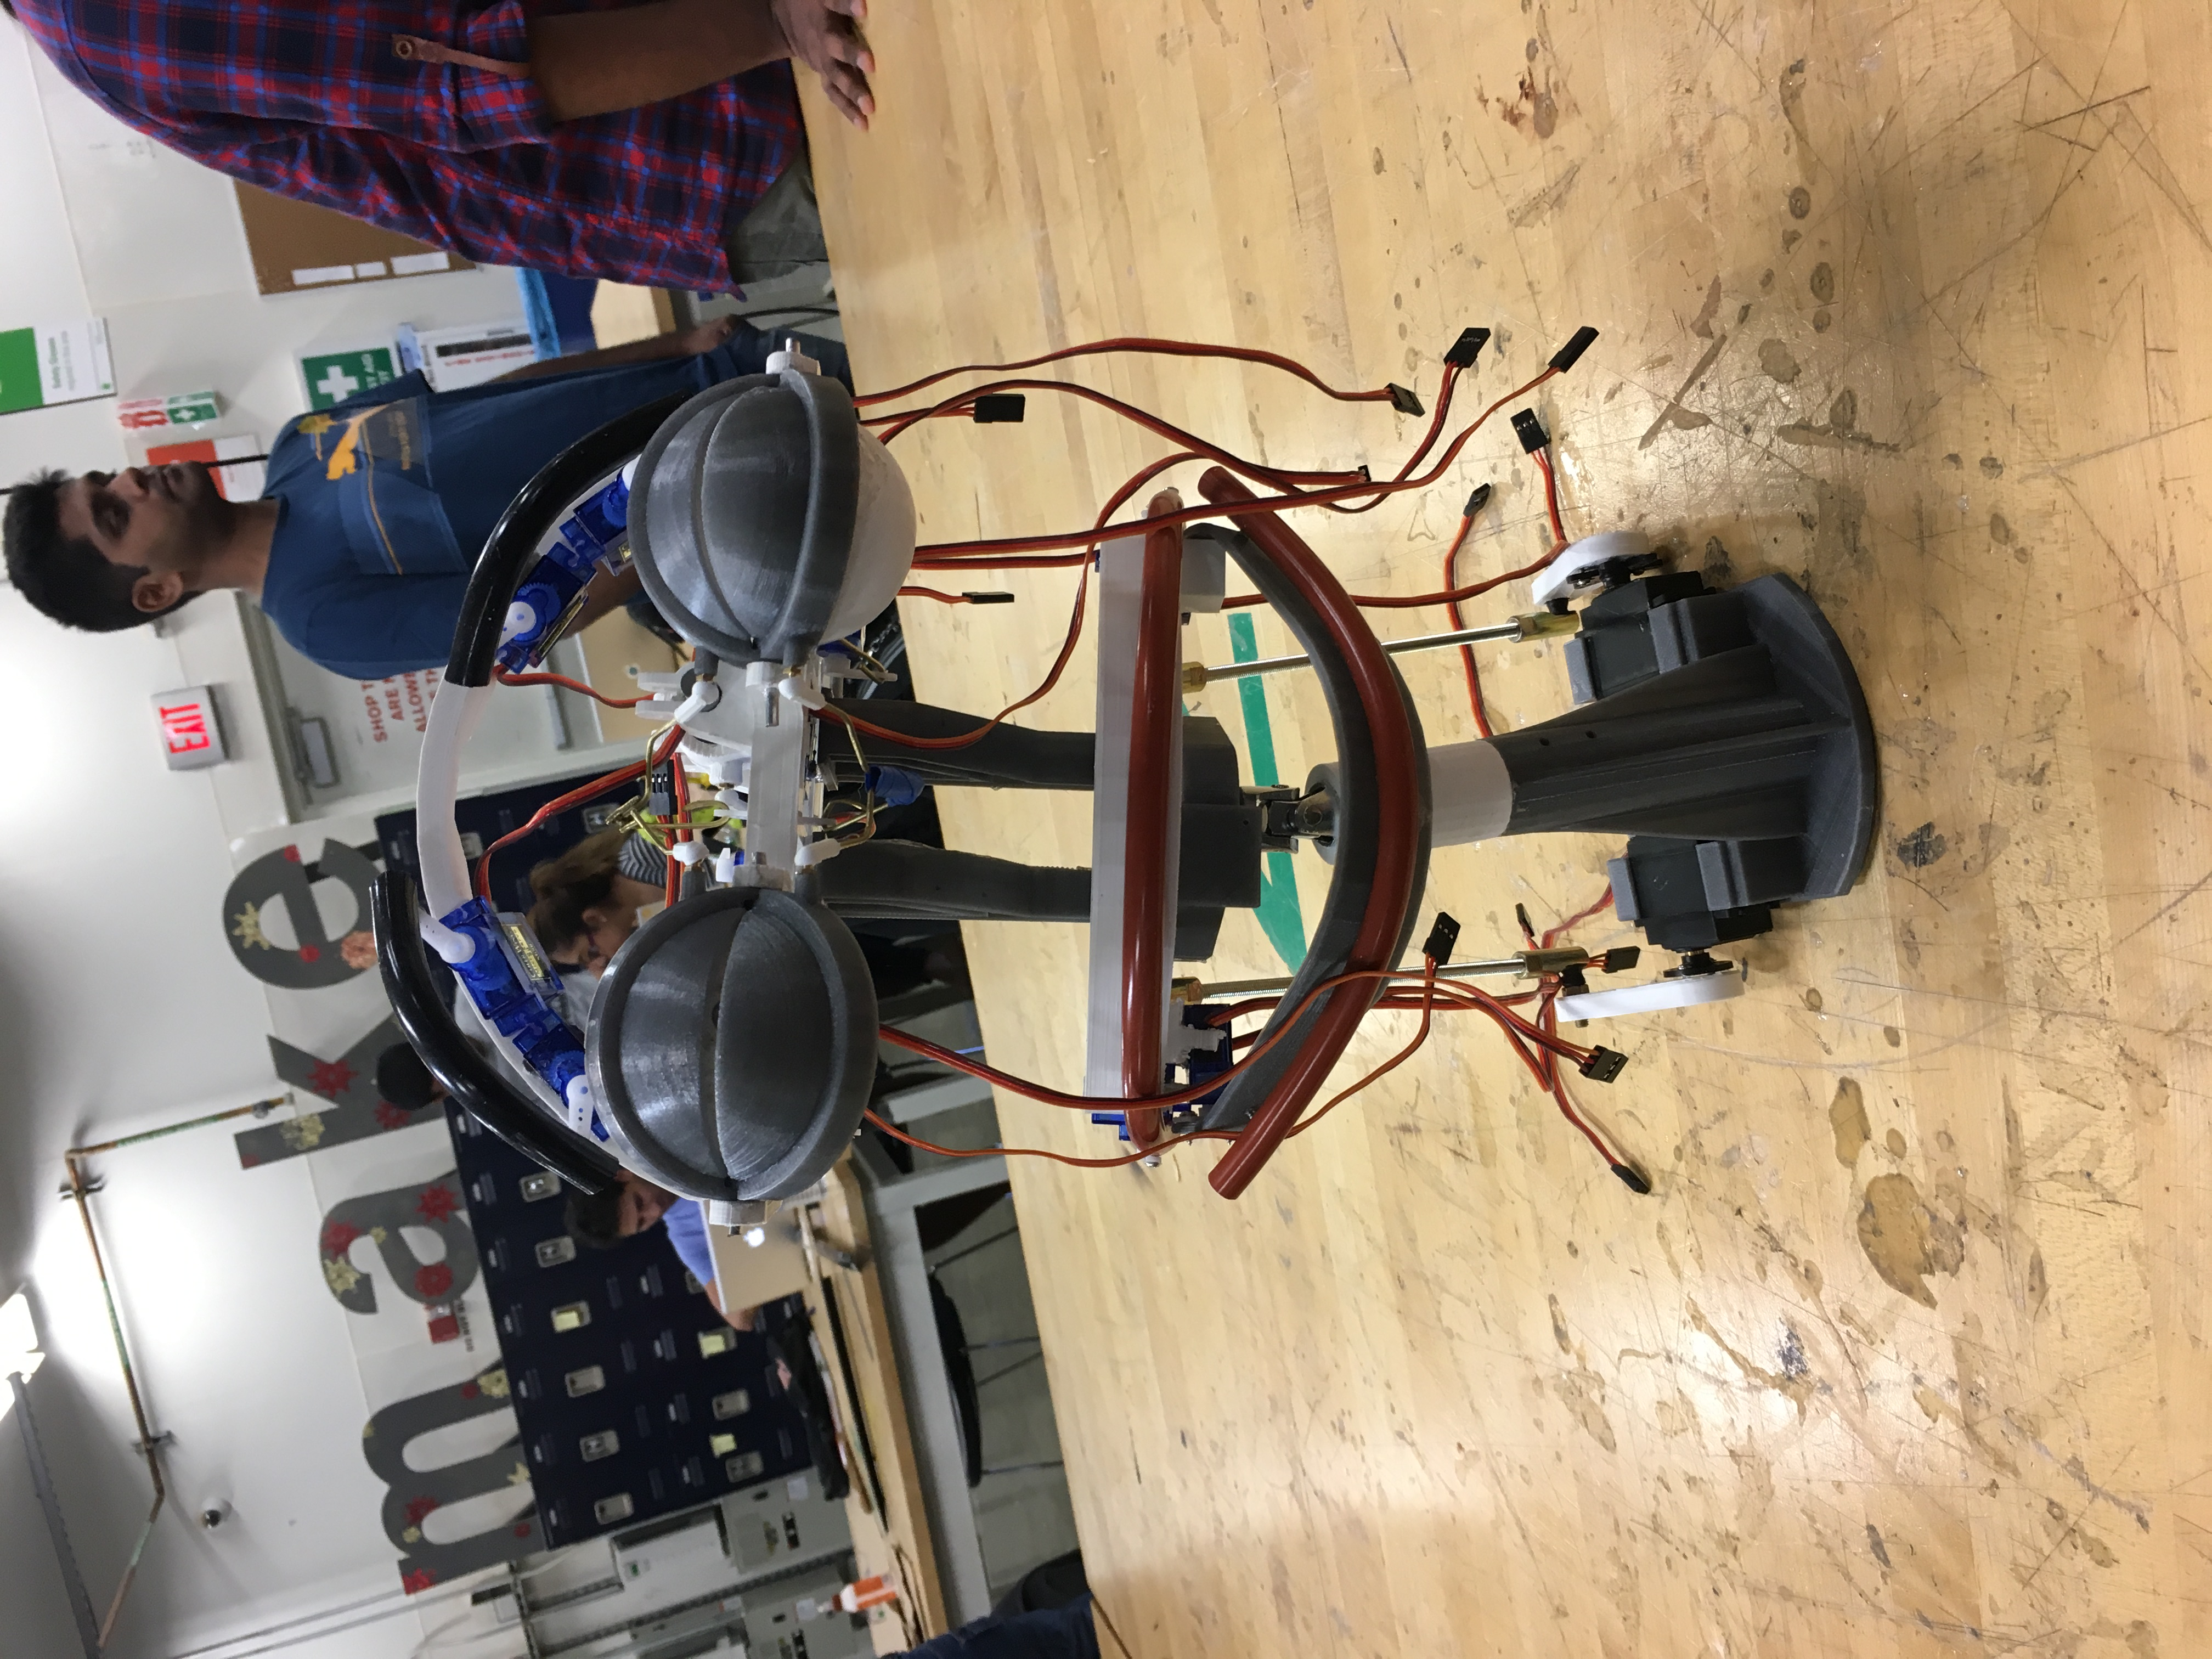
\includegraphics[width=0.3\linewidth, angle=-90]{robot_ready}
\end{center}
\caption{Robot glued together}
\label{fig:robot_ready}
\end{figure}

%----------------------------------------------------------------------------------------

{\let\clearpage\relax \labday{17-26 October 2016}}

\experiment{PSOC Controller and Assembly}
Today, we were introduced to the PSOC controller software which could be used to program the microcontroller. Our professor gave us a walkthrough with the software to make everyone comfortable. We were also given a sample program that could be used to complete the code for rest of the motors. We designed the PWM for all the motors.

\begin{figure}[H]
\begin{center}
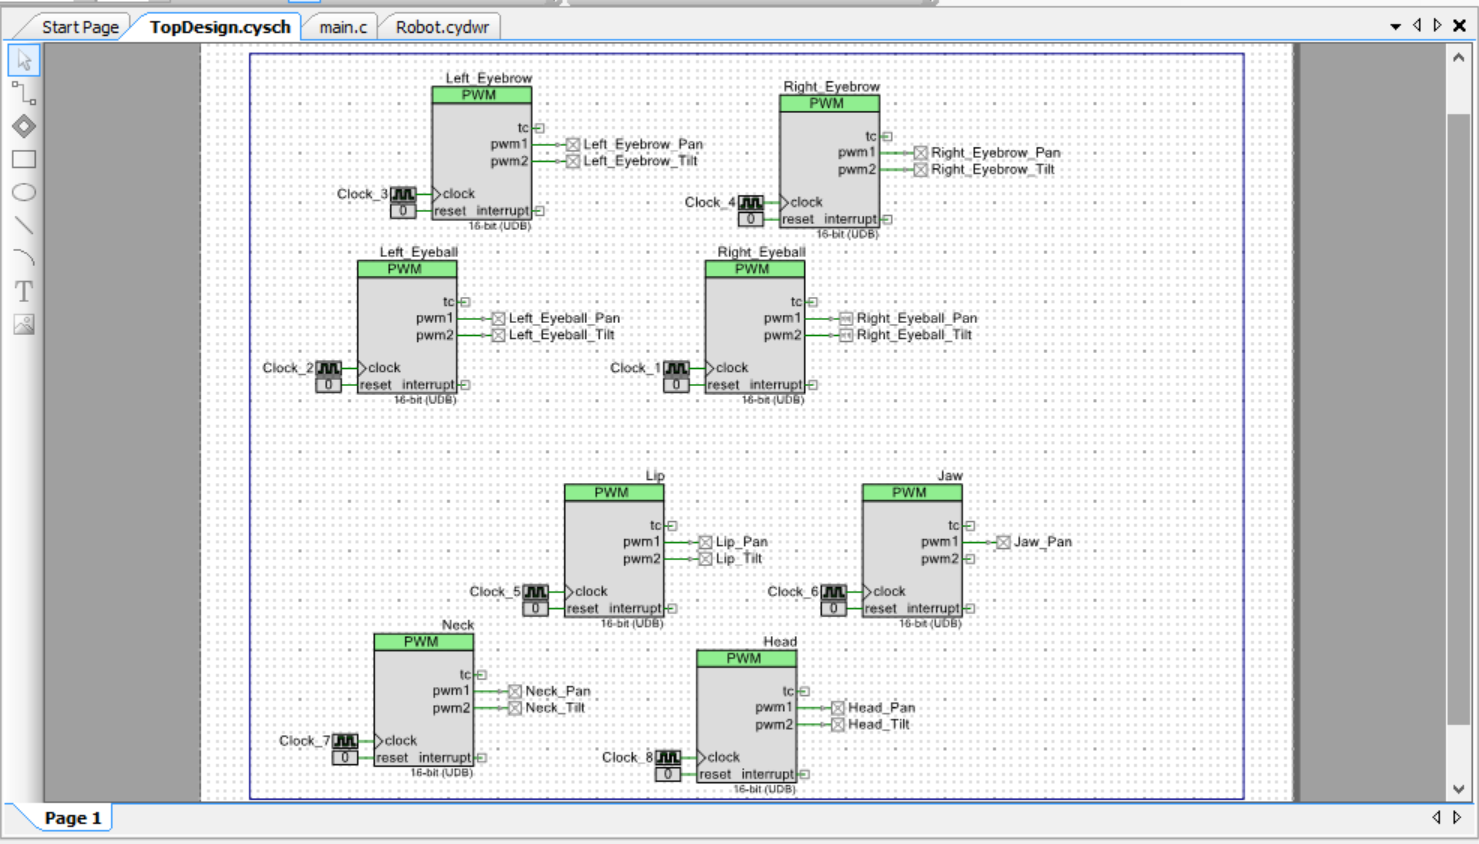
\includegraphics[width=0.8\linewidth]{psoc}
\end{center}
\caption{PSOC Assembly}
\label{fig:psoc}
\end{figure}

%----------------------------------------------------------------------------------------

{\let\clearpage\relax \labday{31 October 2016}}

\experiment{Use Case Tool}
Just like we have github for managing and versioning software code, we were given a presentation by Shawn Pike who developed a Use-Case tool that could be used for software design documents. We were supposed to make small teams that had to consist of an Architect, Solution Manager, Development Manager and Quality Assurance. The use case tool could be used to define use-cases by each of the project role member. New use-cases could be committed by any member and those could be resolved by other members.
\par After the demo of use case tool, we were required to submit a feedback on the design of the tool and the shortcomings that we could find. Personally, I would have found it better if we could give a commit message along with the changes. It gets hard to track the changes otherwise.

%----------------------------------------------------------------------------------------

{\let\clearpage\relax \labday{2 November 2016}}

\experiment{Simulator Experiment - 1}
We got a chance to be a part of an interesting experiment. It was a car simulator and a dashboard layout was being tested. There were 2 layouts, one containing 6 buttons and the other one having 25 buttons. While driving a car, the drivers were being assesed on how fast one could react to a particular layout of the dashboard. The simulator gave a real life like experience of the cars and the vehicles on the road. It was an amazing experience as it gave us an example of how a dashboard can affect driving conditions.

\experiment{Simulator Experiment - 2}
Our professor gave us another opportunity with the driving simulator. This time, we had to experiment with a dashboard app which had several functions like GPS, media player, car functions and driver assist functions. We got a chance to drive under 3 conditions; daytime, night time and a foggy morning. It was amazing to see how certain conditions could affect the reaction time for a driver using an application on the dashboard.

\begin{figure}[H] % Example of including images
\begin{subfigure}{.5\textwidth}
  \centering
  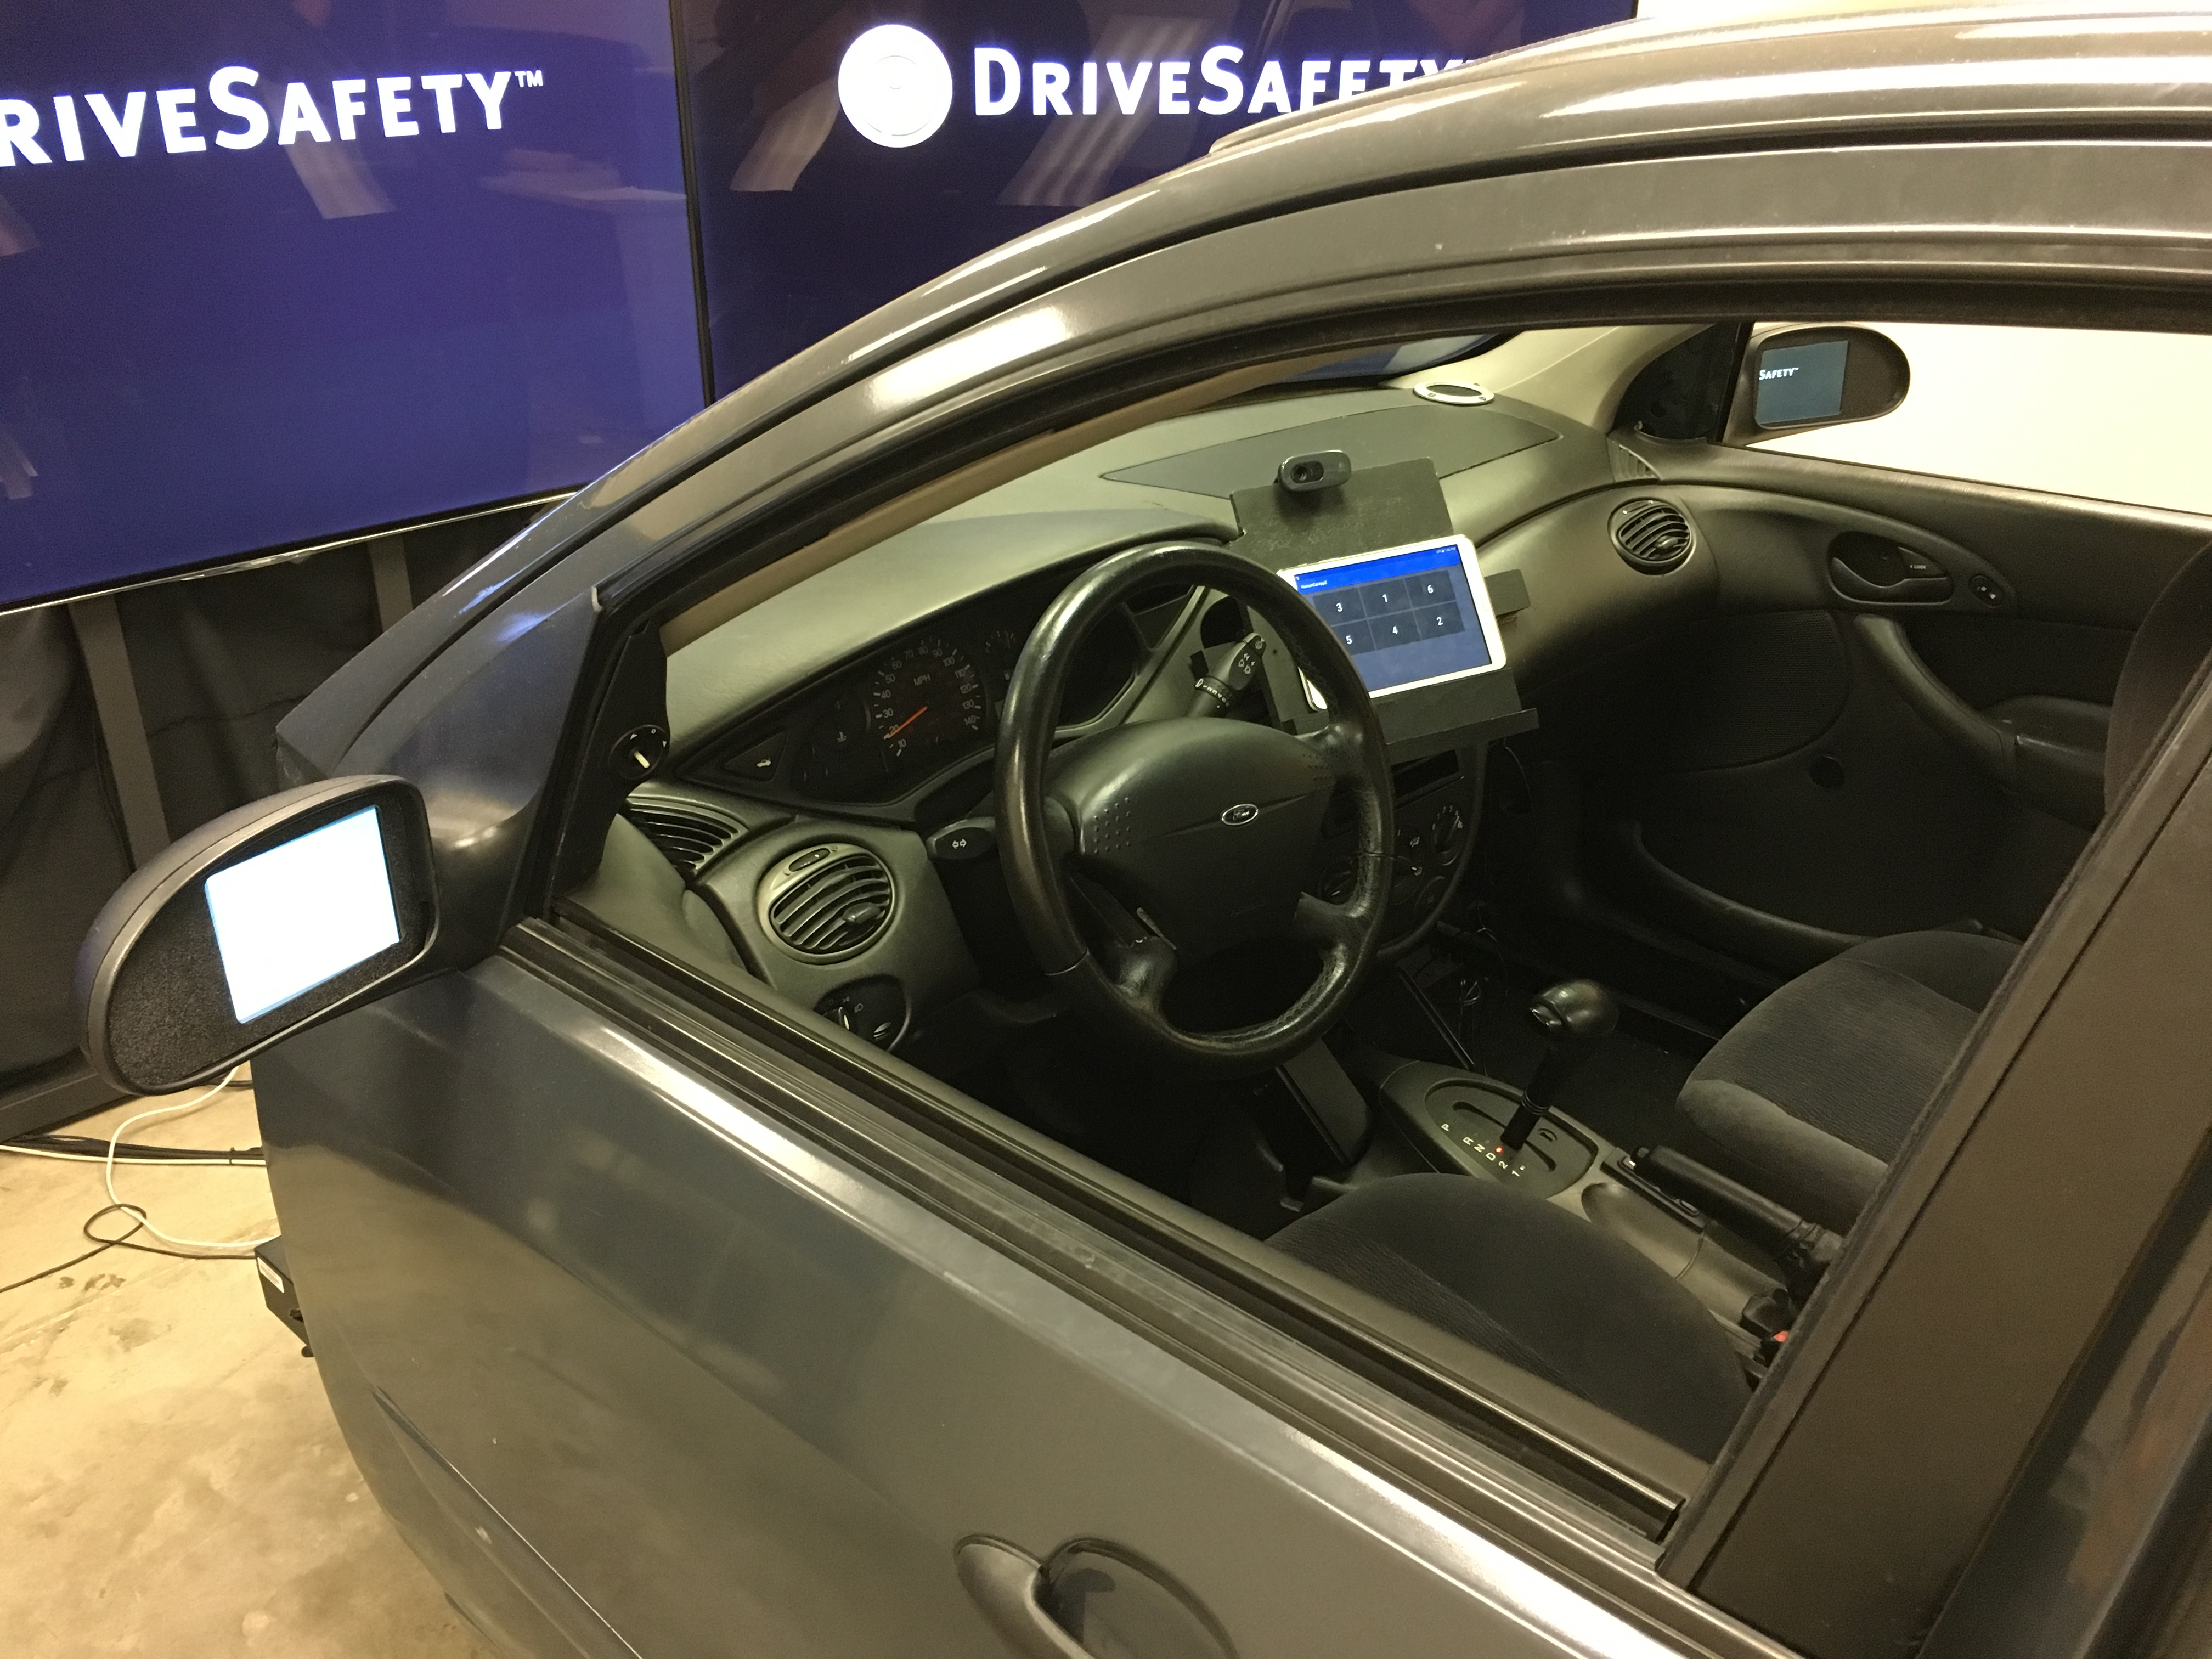
\includegraphics[width=.65\linewidth]{simulator_car}
  \caption{Car Simulator}
  \label{fig:simulator_car}
\end{subfigure}%
\begin{subfigure}{.5\textwidth}
  \centering
  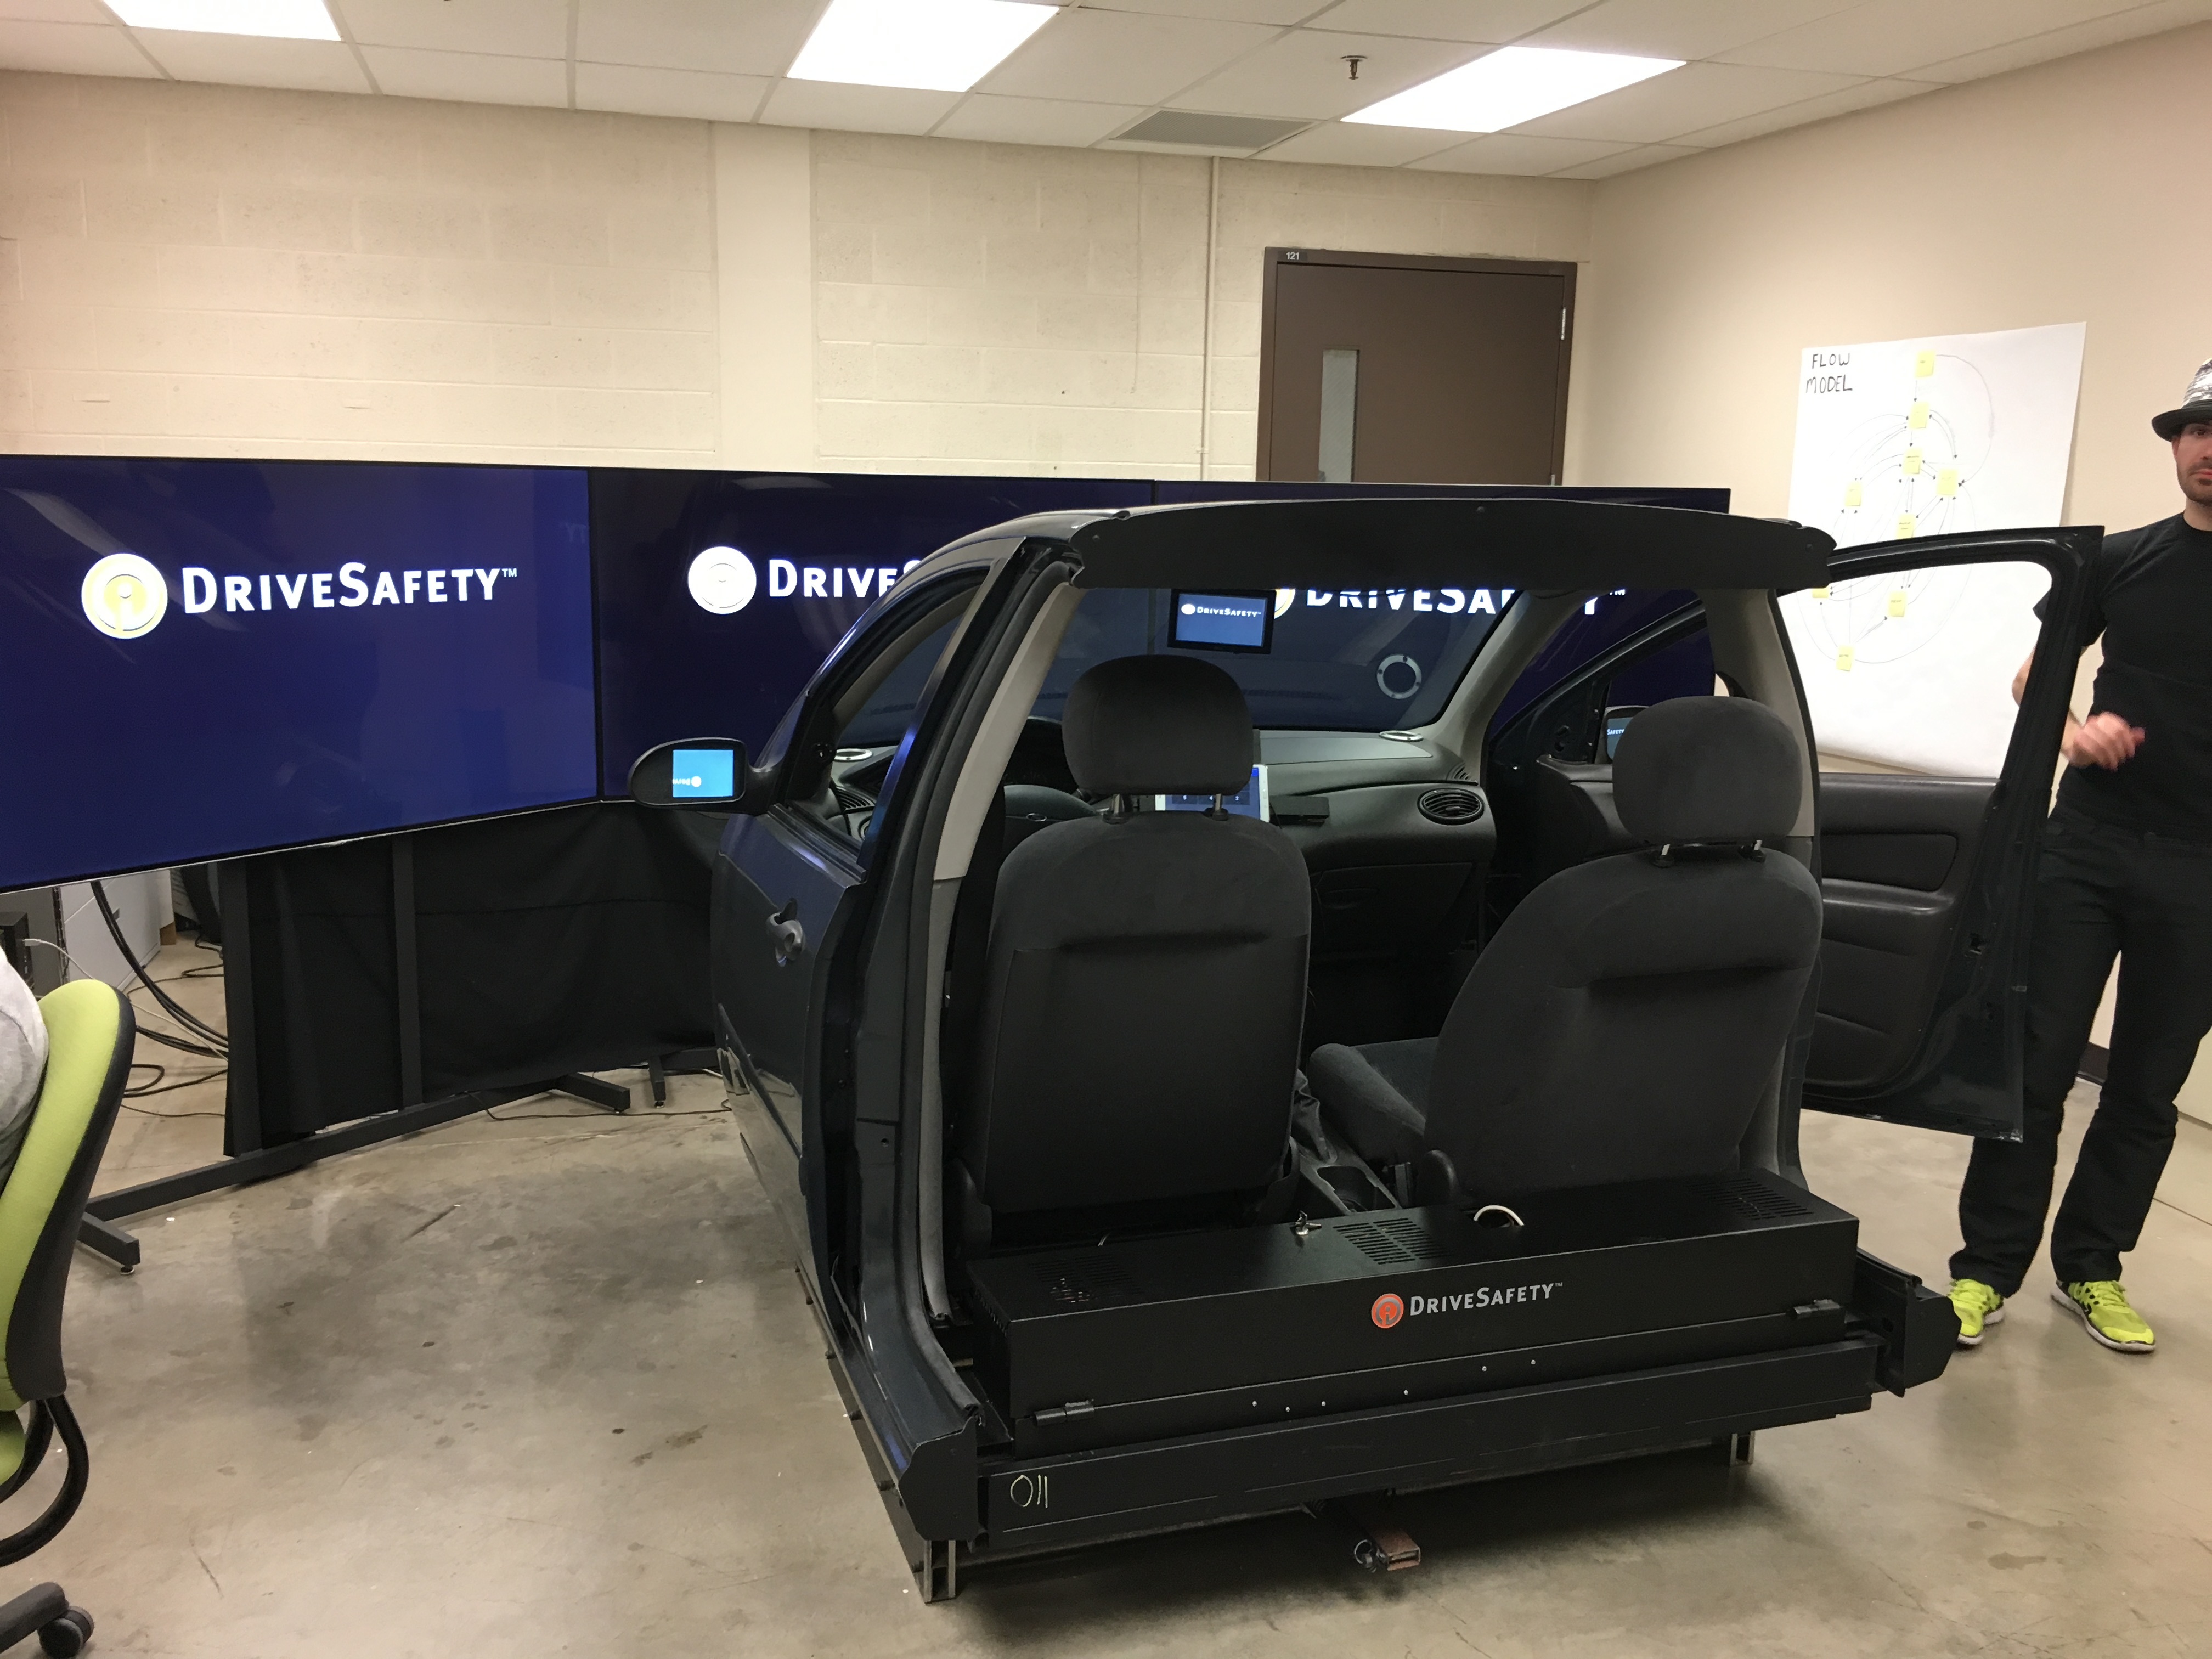
\includegraphics[width=.65\linewidth]{simulator_setup}
  \caption{Car simulator setup}
  \label{fig:simulator_setup}
\end{subfigure}
\label{fig:servo_motors}
\end{figure}

%----------------------------------------------------------------------------------------

{\let\clearpage\relax \labday{7,9 November 2016}}

\experiment{Wiring of the robot}
To start wiring the robot, we needed to have a blueprint of the design such that every team member could be in sync with the wires. Each motor was assigned a number and for each motor we had 3 wires; positive, negative and the controlling wire. The numbers on the left column represented the rows on the breadboard. For each row we had 3 wires which controlled the motors.

\begin{figure}[H]
\begin{center}
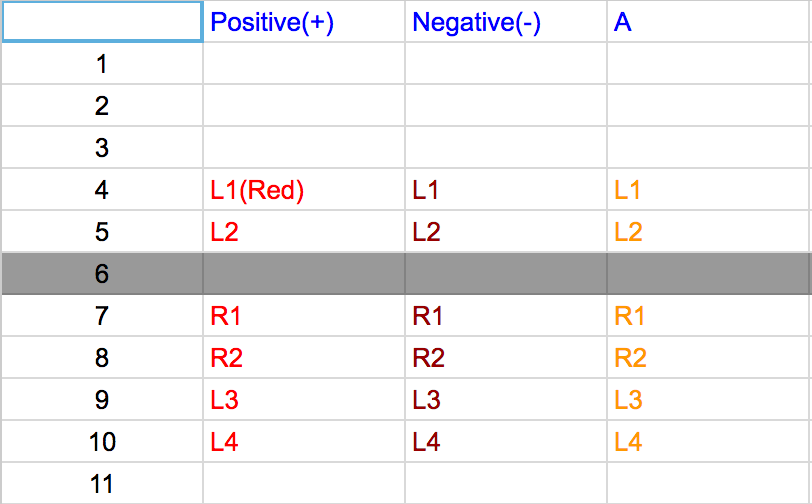
\includegraphics[width=0.4\linewidth]{wiring_blueprint}
\end{center}
\caption{Sample blueprint of wiring}
\label{fig:wiring_blueprint}
\end{figure}

\experiment{Connecting the wires}
We labeled each motor in sync with the blueprint. This would make it easy to refer to the motors and we would not have to backtrack each of the wire.
\begin{figure}[H] % Example of including images
\begin{subfigure}{.5\textwidth}
  \centering
  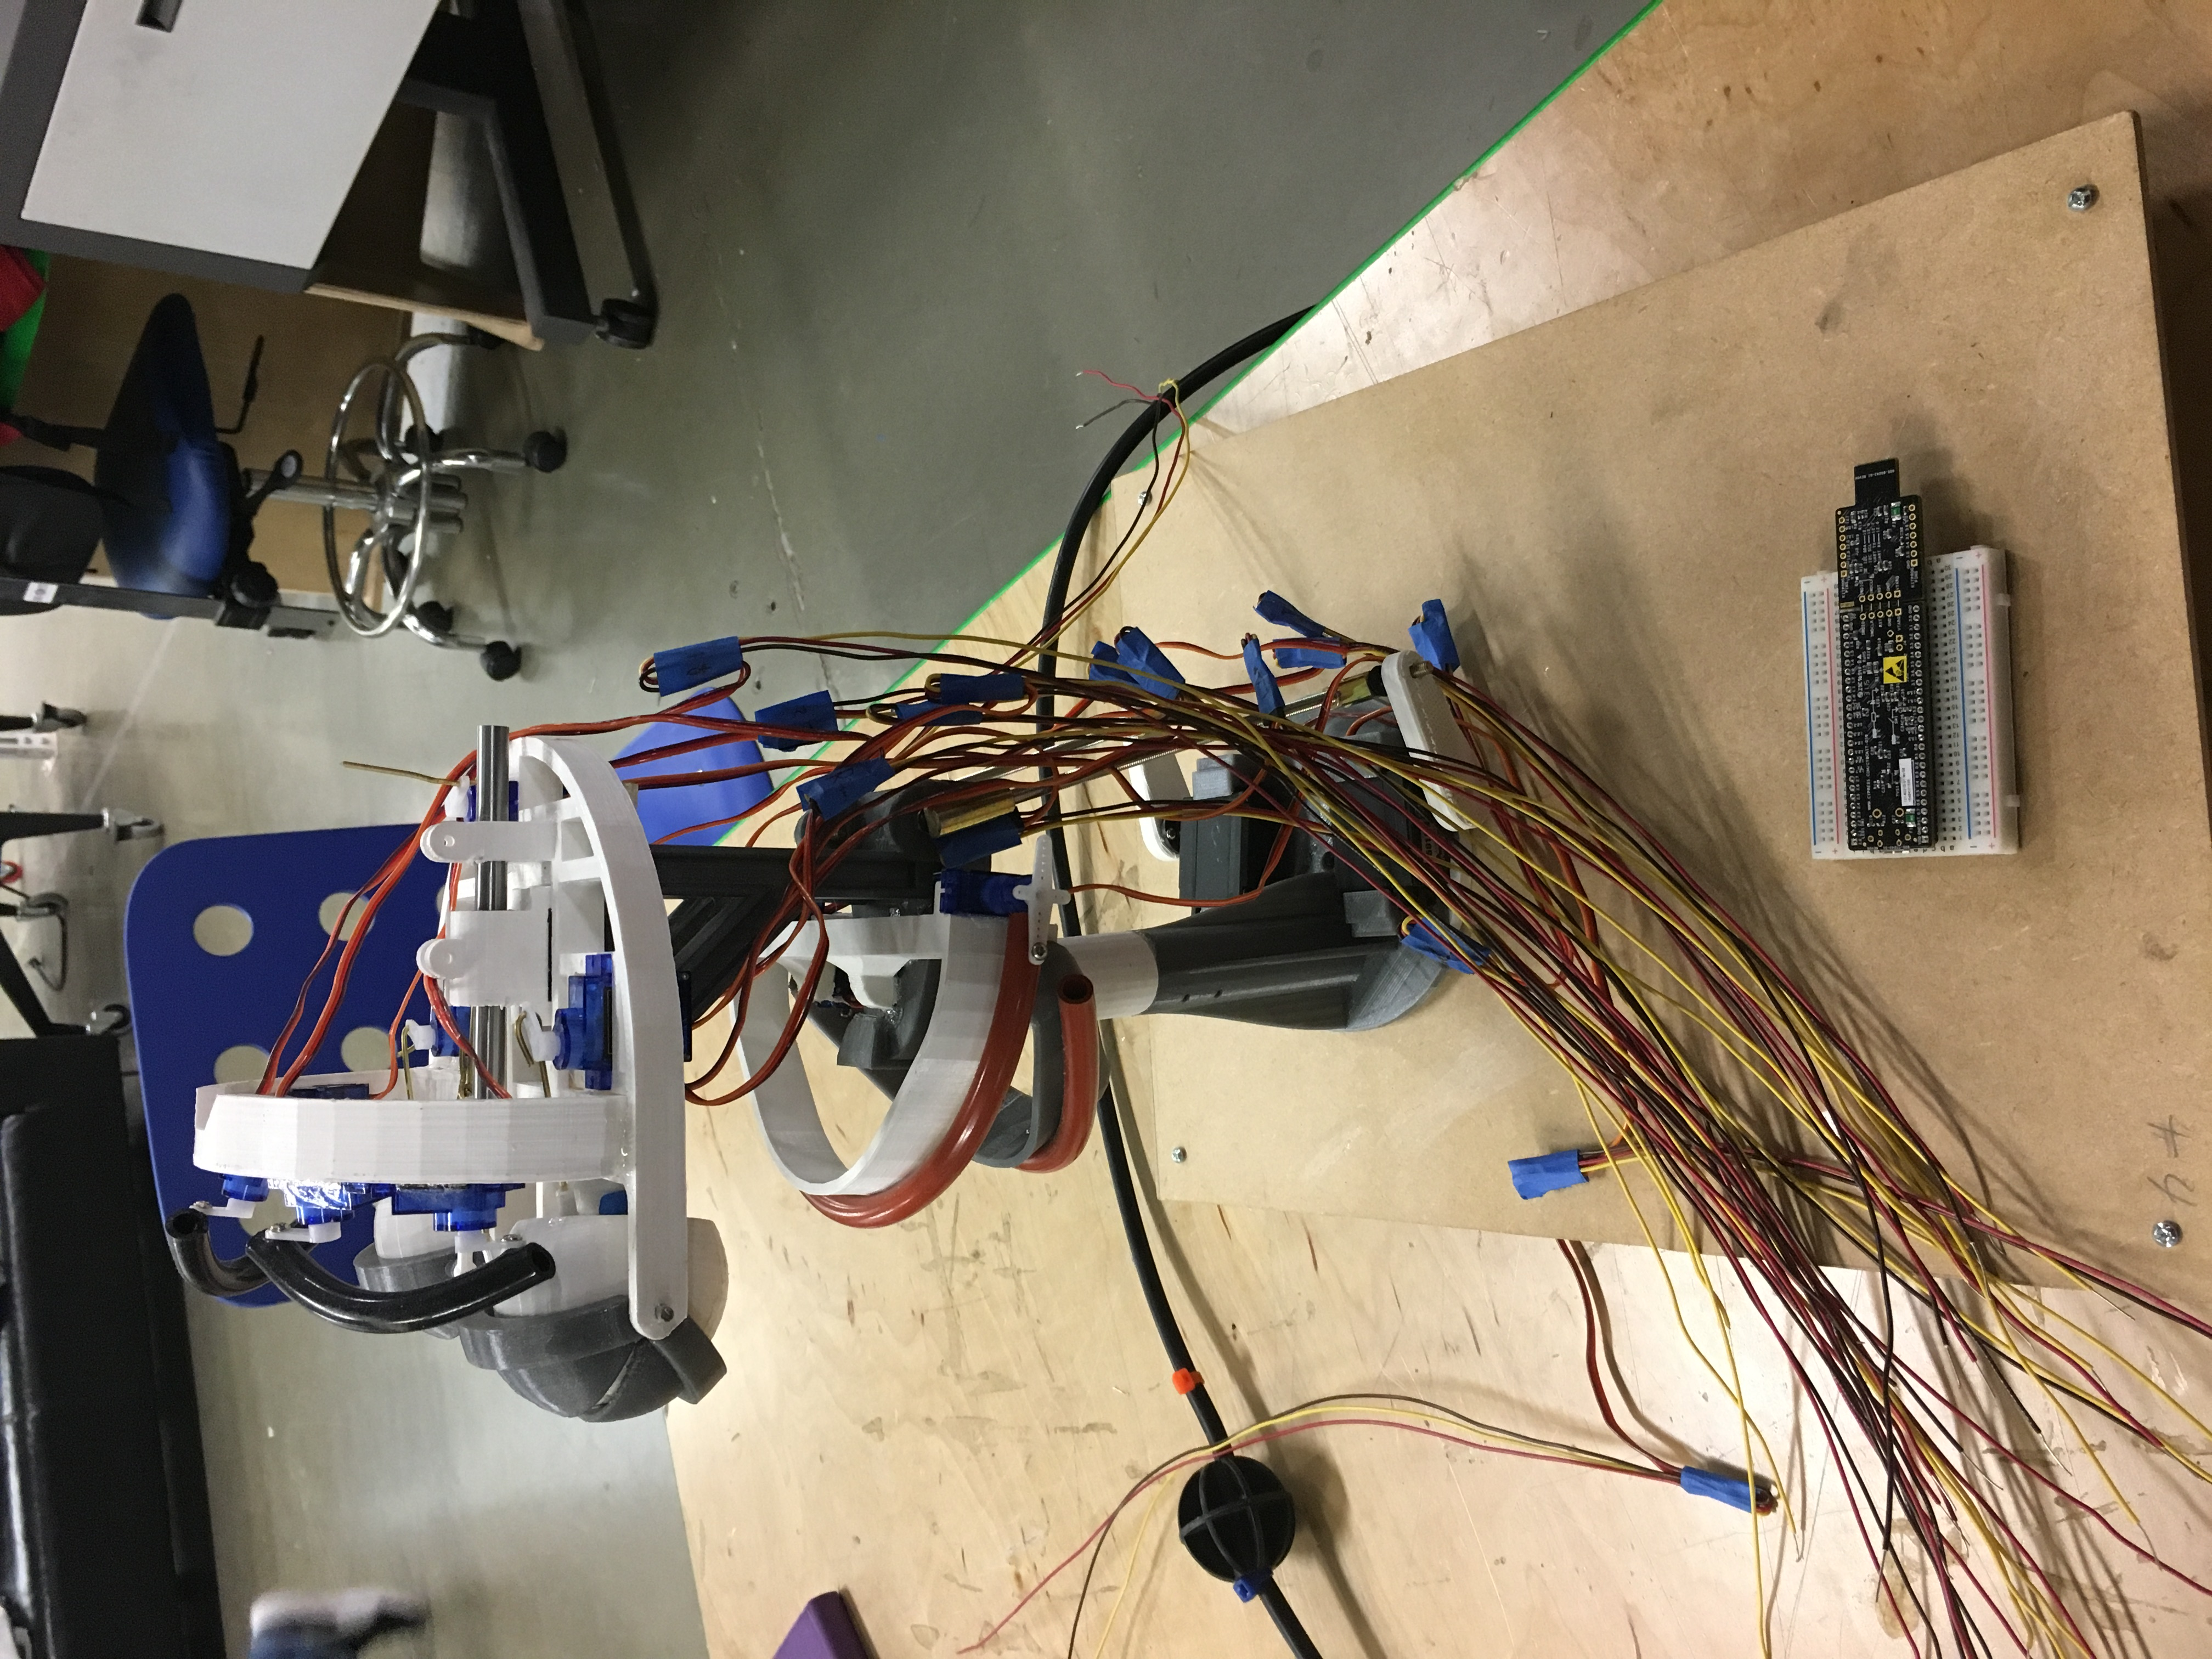
\includegraphics[width=.65\linewidth, angle=-90]{robot_wiring_complete}
  \caption{Robot wiring with labels}
  \label{fig:robot_wiring_complete}
\end{subfigure}%
\begin{subfigure}{.5\textwidth}
  \centering
  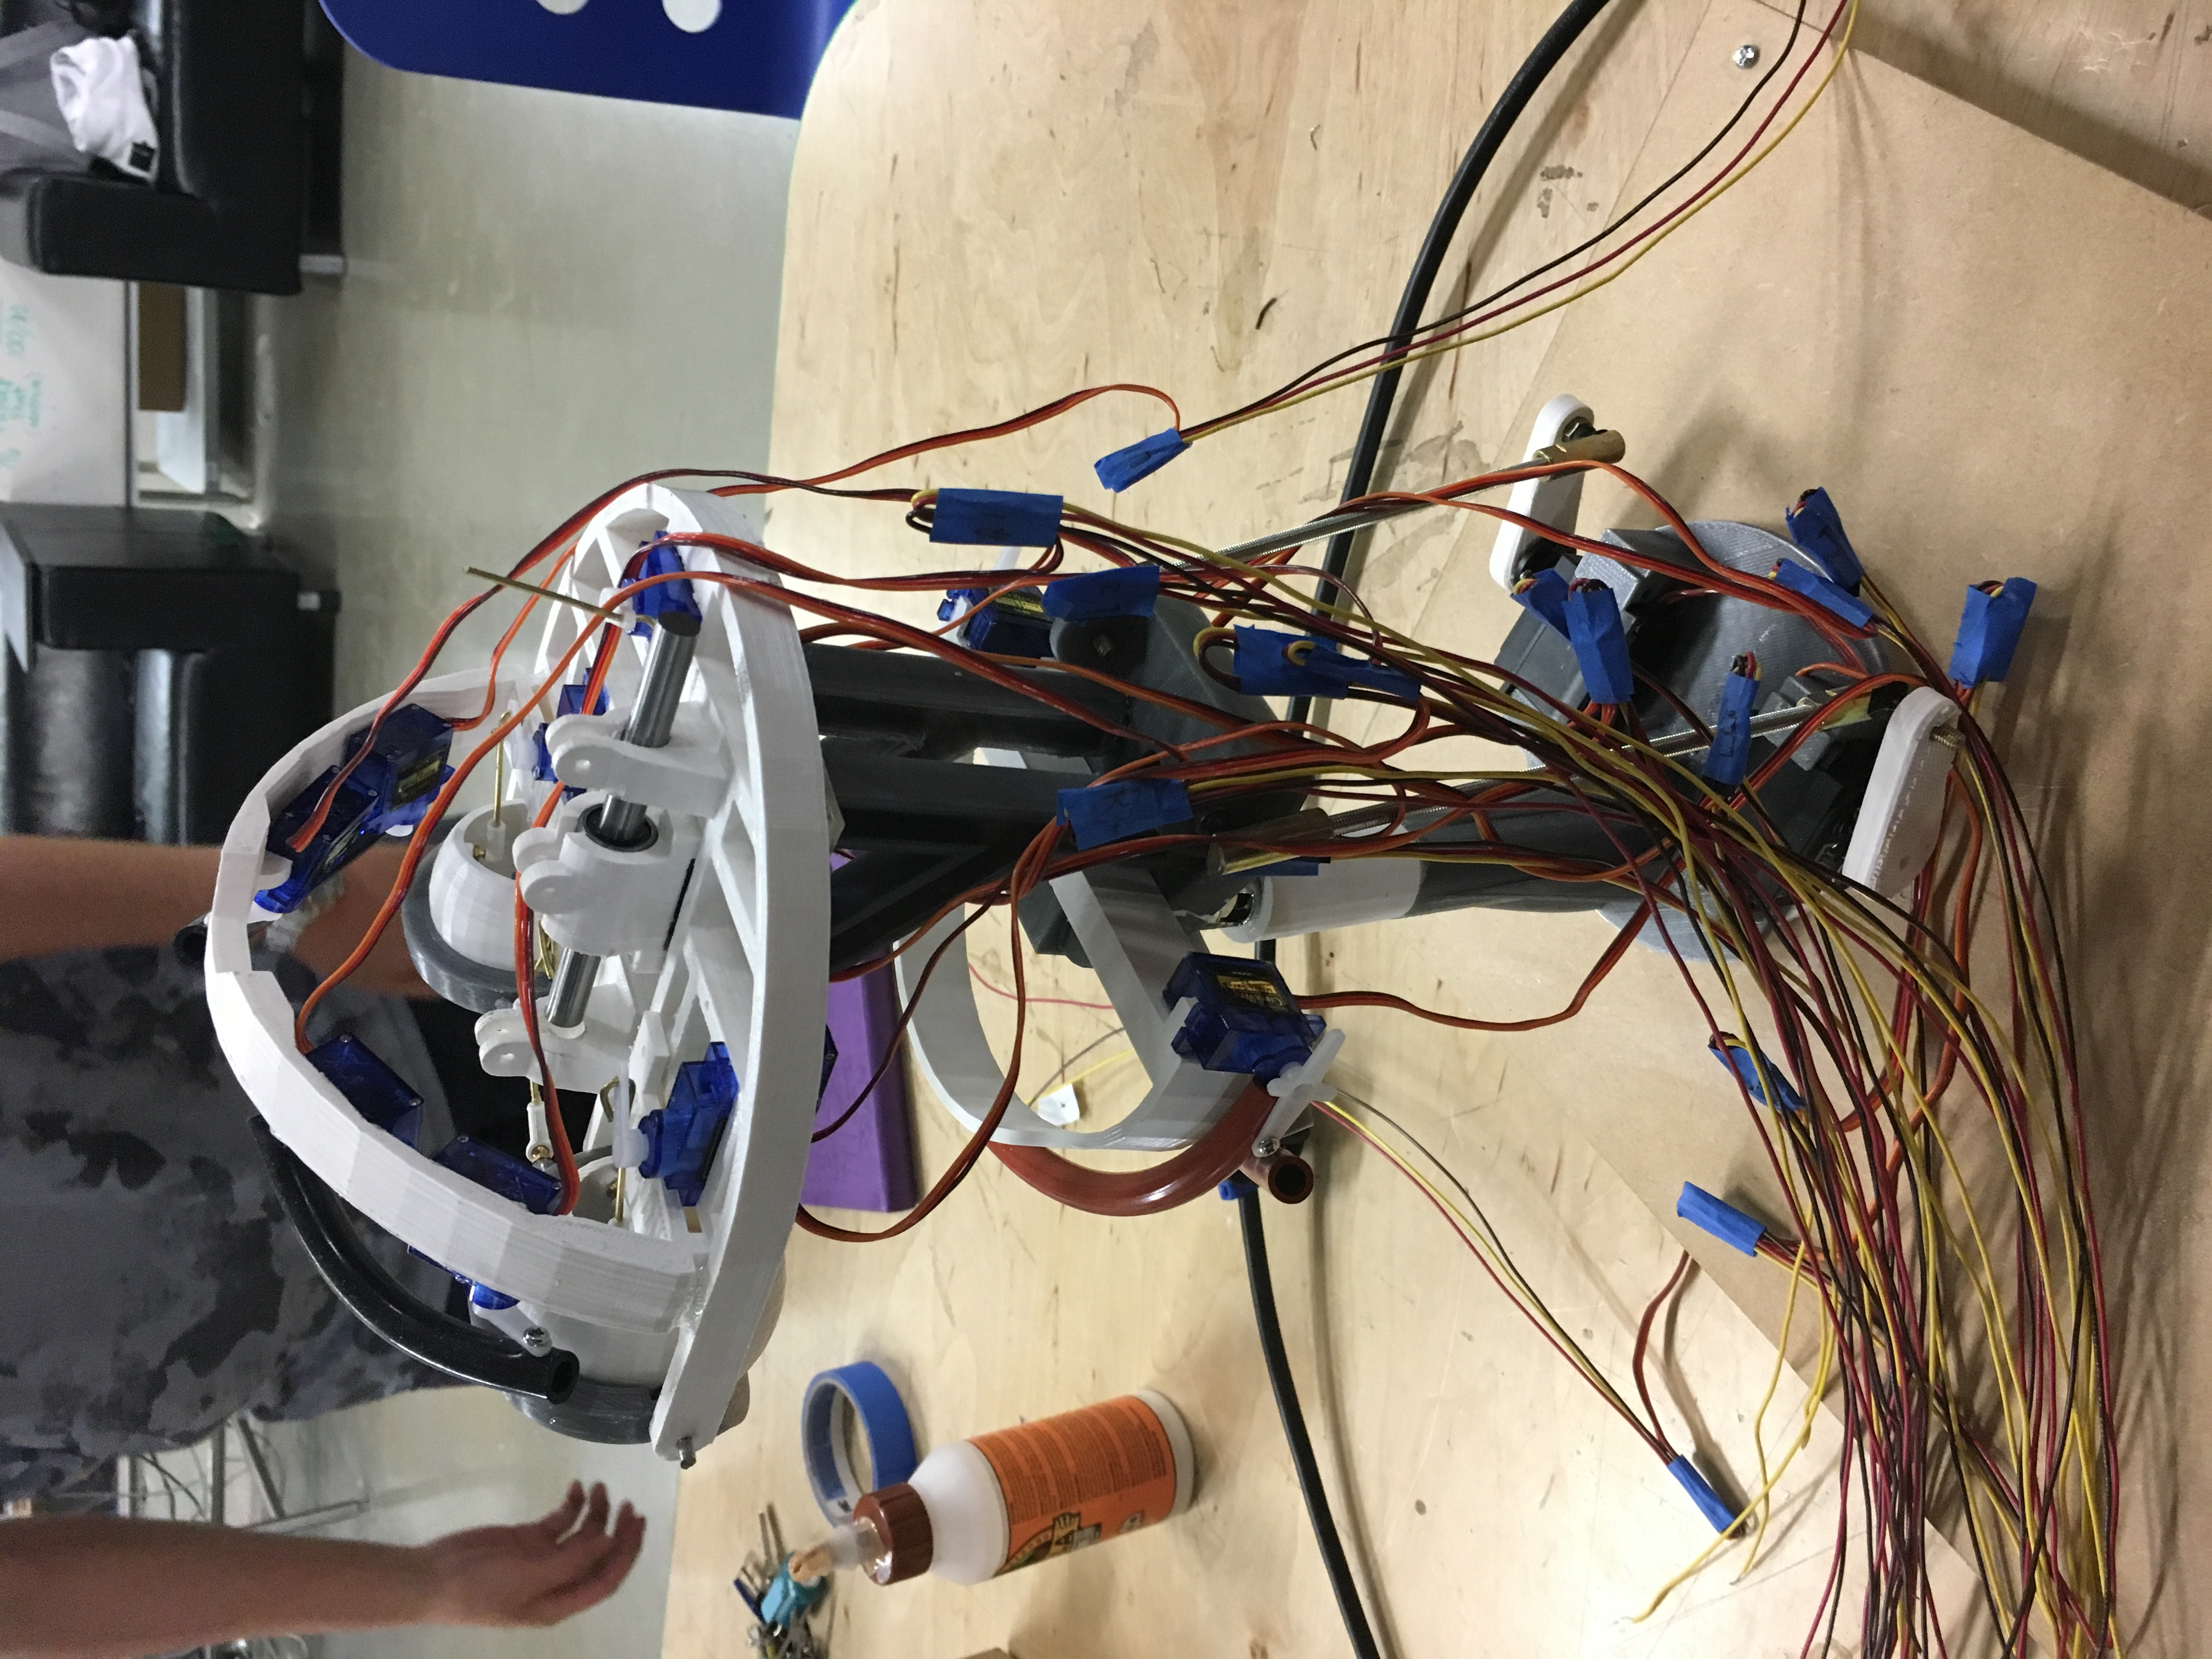
\includegraphics[width=.65\linewidth, angle=-90]{wiring_backside}
  \caption{Wiring back side}
  \label{fig:wiring_backside}
\end{subfigure}
\caption{Wiring the robot}
\label{fig:servo_motors}
\end{figure}

\experiment{Robot moved for the first time}
We had the PWM's in place, all the wiring correctly in place, and the robot all ready. It was time to test the robot. We programmed the microcontroller, placed it on the breadboard and connected the wires. The robot came to life and it made its first gesture.

\begin{figure}[H]
\begin{center}
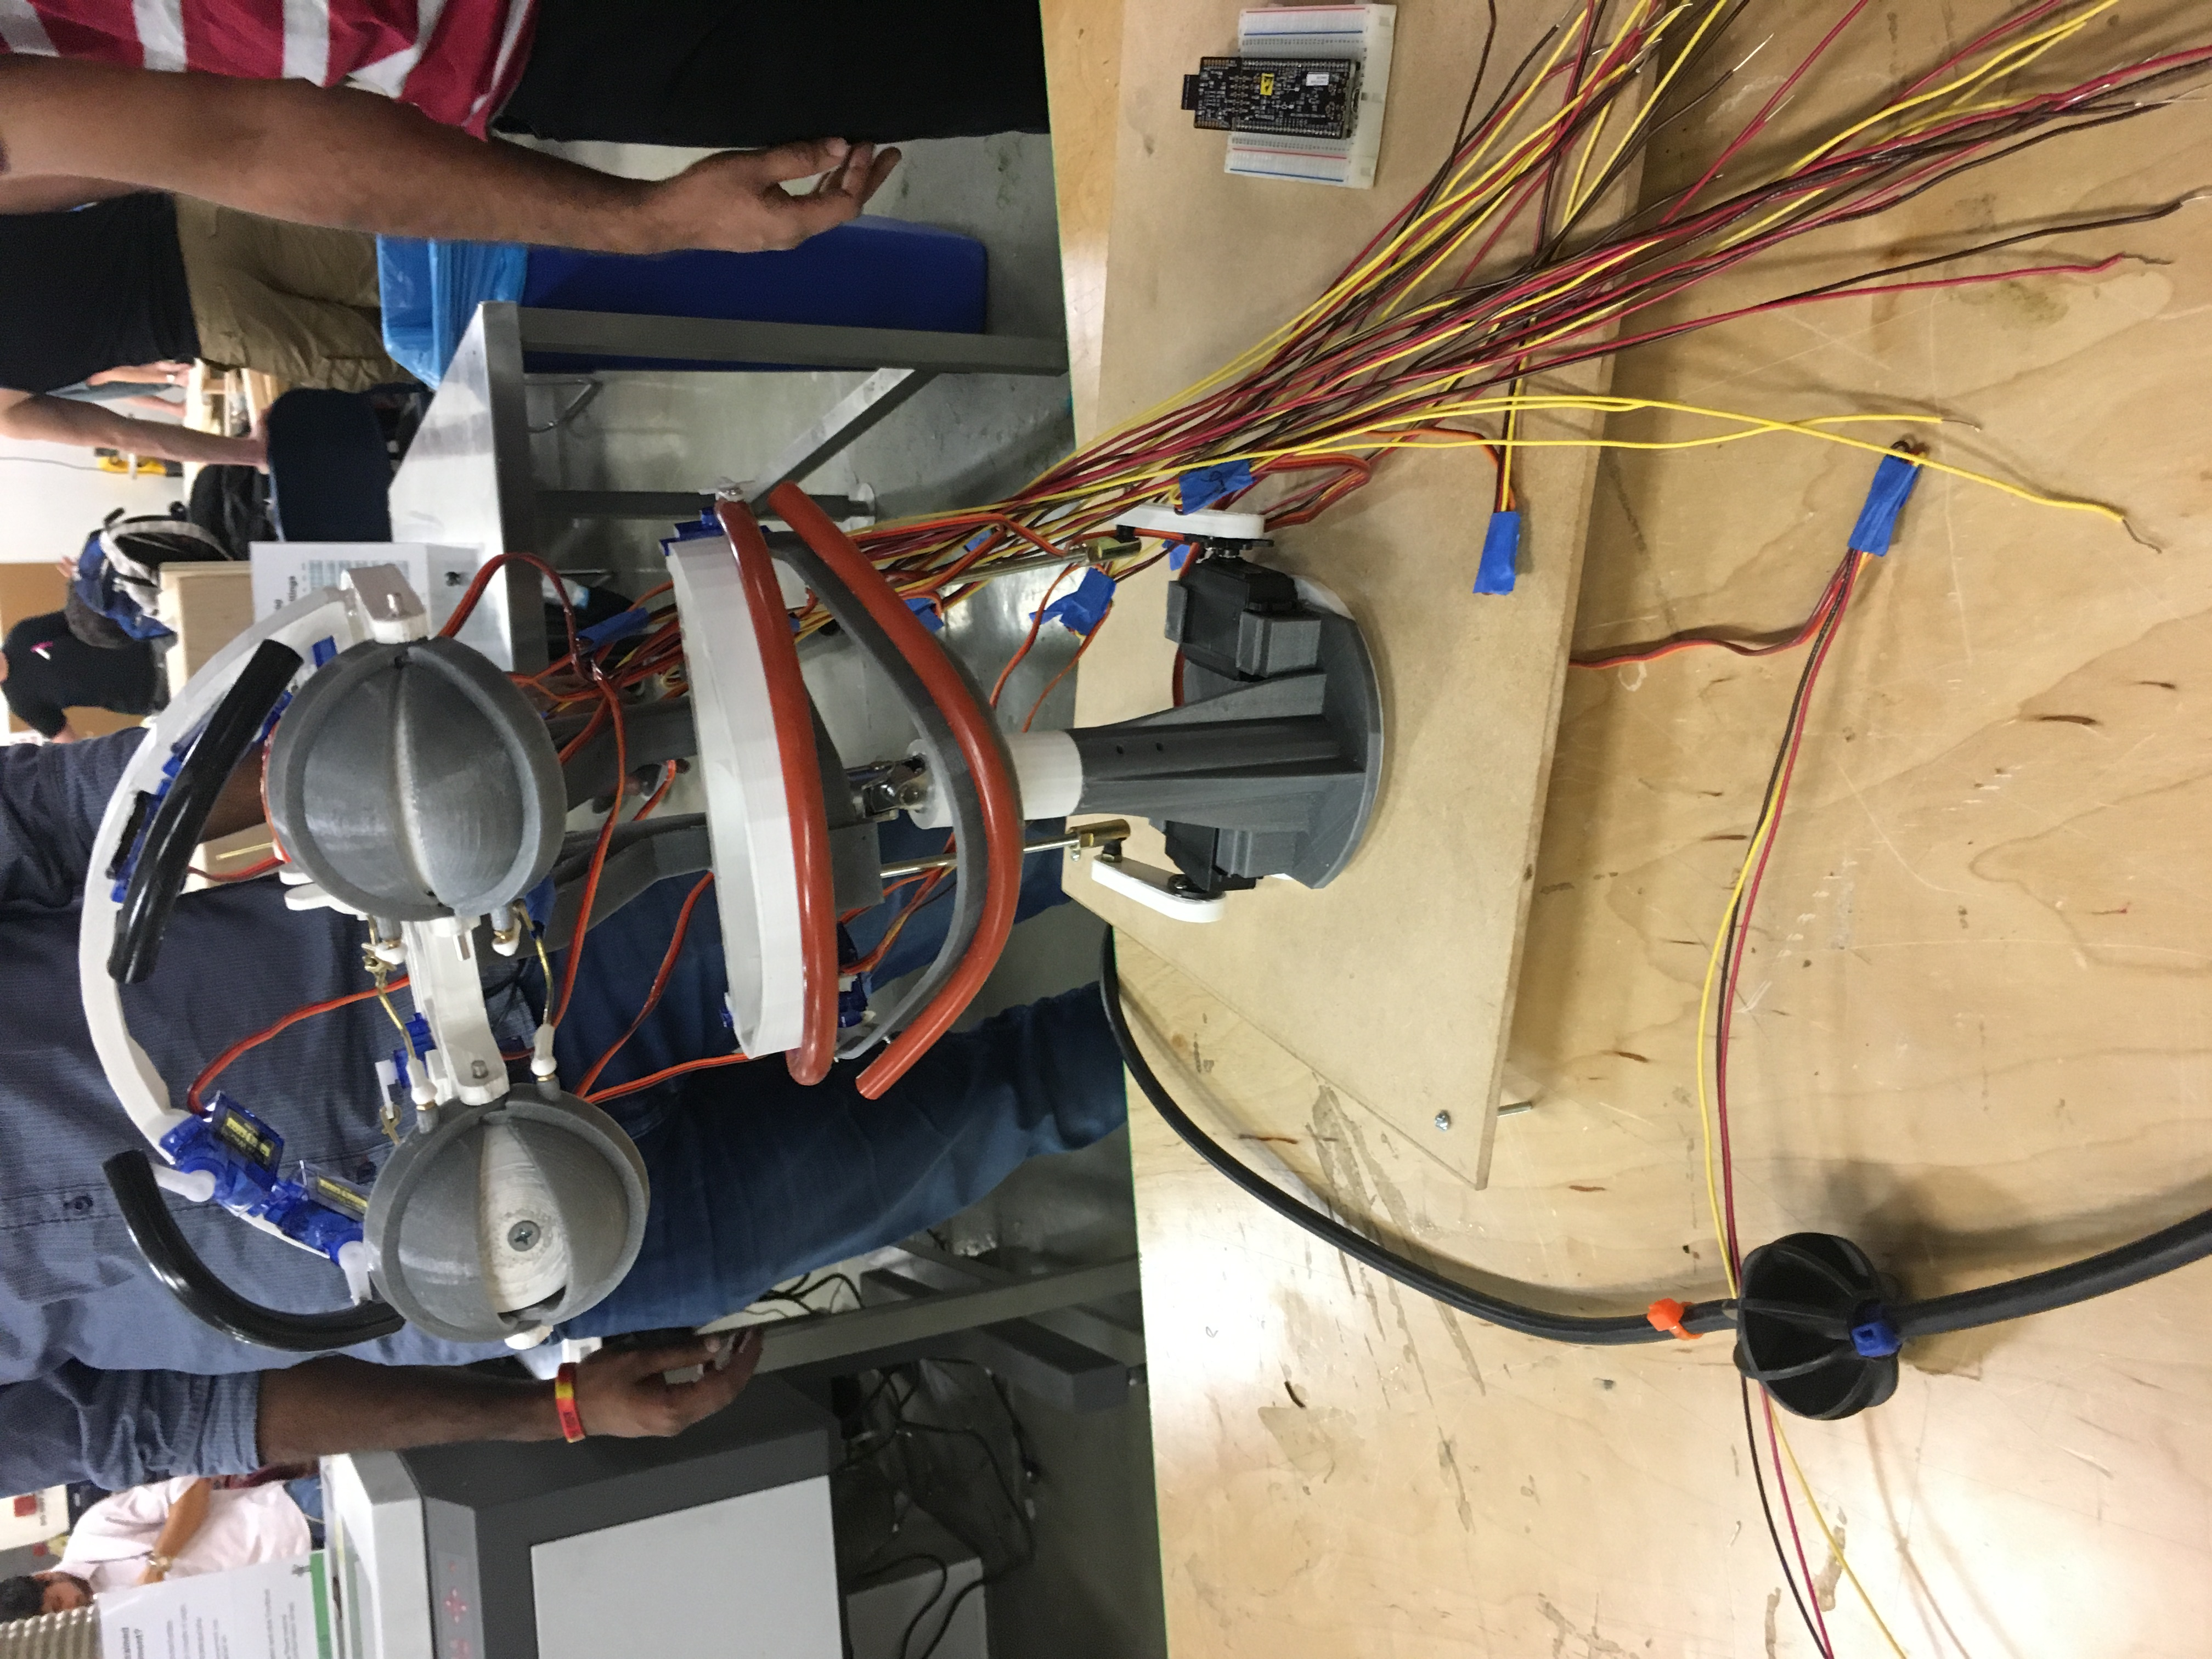
\includegraphics[width=0.4\linewidth, angle=-90]{the_first_movement}
\end{center}
\label{fig:the_first_movement}
\end{figure}

%----------------------------------------------------------------------------------------

{\let\clearpage\relax \labday{14-30 November 2016}}

\experiment{Class Instructions on Topic Demo}
Each of the 8 teams were assigned certain topics to give a presentation. These topics were related to some of the latest trends in the current software industry. The notable topics being Mental Modeling, Story Boarding, Artifical Intelligence, User Center Design, Autonomous Cars etc. Our team got a topic of Mental Modeling. The professor explained how to go about the presentation and what points we had to focus on. The slides was supposed to contain a lot many images and bullet points while we were required to describe the details during presentation.
\par Our professor gave us a very good example of Ford, and how they used the assembly line to make the manufacturing process easier. We also discussed the design idea of Tesla motors and how they are using it to make autonomous cars. The class discussions were very helpful to understand which areas to research upon.
\par Meanwhile, we started preparing our presentation on Mental Modeling. We also had a small demo of the work done so far, and our professor gave us more insights of coming up with more examples.

\experiment{Topic Demos}
This was the presentation week and every team started giving the description of their respective topics. We learned that strategising a presentation is as important as actually describing it. Our professor laid emphasis on the fact that we have exactly 10 minutes in a presentation and not a second extra. What we speak should be concise and descriptive at the same time.
\par We also gave our presentation on Mental Modeling in groups of 2 which the professor really appreciated. While giving the presentation our professor also gave us various examples how mental modeling is being used in everyday life. He emphasized on the fact that we need mental modeling to maintain a consistency between the designer, developer and the end user.

%----------------------------------------------------------------------------------------

{\let\clearpage\relax \labday{4 December 2016}}

\experiment{Completing the robot and expressions}
We met at a common place, a team member's house to complete the robot expressions and all the programming. The classes were over and we had to take out some extra time to complete all the deliverables. Our microcontroller seemed to blow up at one instance which got us worried and we started to look for a new one. However, after several iterations and connections the microcontroller somehow started working again which was a relief. We programmed several expressions of the robot with its eyes and its jaws.\\ \\
- Jaw Dropping Expression\\
- Twirling Eyebrows\\
- Grim smile\\

%----------------------------------------------------------------------------------------
\end{document}